\documentclass[8pt]{extarticle}
\usepackage{fix-cm}

% Packages
\usepackage{geometry}
\usepackage{multicol}
\usepackage[dvipsnames]{xcolor}
\usepackage{colortbl}
\usepackage{graphicx} % Required for inserting images
\usepackage{amsmath}
\usepackage{amssymb}
\usepackage{enumerate}
\usepackage{soul}
\usepackage{tikz}
\usepackage{tcolorbox}

%%%% Smaller Spacing
% --- FONT SIZE OVERRIDE ---
\usepackage{scrextend}
\changefontsizes{6pt} 

\linespread{0.7} % Very tight line spacing

% make itemize use less space
\usepackage{enumitem}
\setlist[itemize]{noitemsep, topsep=0pt}
\setlist[enumerate]{noitemsep, topsep=0pt}

% Remove titlespacing
\usepackage{titlesec}
\titlespacing*{\section}
{0pt}{1.2ex}{0.8ex}

\titlespacing*{\subsection}
{0pt}{1.0ex}{0.6ex}

\titlespacing*{\subsubsection}
{0pt}{2.0ex}{0.4ex}

%--------------------------------------------------------
%
\titleformat{\section}
  {\fontsize{9pt}{11pt}\selectfont\bfseries\color{teal}}
  {\thesection}{1em}{}

\titleformat{\subsection}
  {\fontsize{8pt}{10pt}\selectfont\bfseries\color{red}}
  {\thesubsection}{1em}{}

% Layout
\geometry{a4paper, landscape, margin=6.67mm}
\setlength{\columnsep}{6.67mm}
\setlength{\columnseprule}{.33pt}
\setlength{\parindent}{0pt}
% Images
\graphicspath{ {./images/} }
% Commands
\newcommand*{\vertbar}{\rule[-1ex]{0.5pt}{2.5ex}}
\newcommand*{\horzbar}{\rule[.5ex]{2.5ex}{0.5pt}}


\title{Linare Algebra: Cheat Sheet}
\author{Cedric Bolleter}
\date{January 2026}

\begin{document}
\begin{multicols*}{4}

\newtcbox{\yellowBox}{
    on line,
    colback=yellow!100,
    colframe=yellow!0,
    arc=3pt,
    boxrule=0pt,
    left=0pt,right=0pt,top=-1pt,bottom=-1pt
}

\newtcbox{\orangeBox}{
    on line,
    colback=orange!55,
    colframe=orange!0,
    arc=3pt,
    boxrule=0pt,
    left=0pt,right=0pt,top=-1pt,bottom=-1pt
}

\newtcbox{\blueBox}{
    on line,
    colback=blue!45,
    colframe=blue!0,
    arc=3pt,
    boxrule=0pt,
    left=0pt,right=0pt,top=-1pt,bottom=-1pt
}

\newtcbox{\lightBlueBox}{
    on line,
    colback=blue!25,
    colframe=blue!0,
    arc=3pt,
    boxrule=0pt,
    left=0pt,right=0pt,top=-1pt,bottom=-1pt
}

\newtcbox{\greenBox}{
    on line,
    colback=green!55,
    colframe=green!0,
    arc=3pt,
    boxrule=0pt,
    left=0pt,right=0pt,top=-1pt,bottom=-1pt
}

\newtcbox{\redBox}{
    on line,
    colback=red!55,
    colframe=red!0,
    arc=3pt,
    boxrule=0pt,
    left=0pt,right=0pt,top=-1pt,bottom=-1pt
}


\newcommand{\definition}[1]{
    \orangeBox{\textbf{#1}}
}

\newcommand{\lemma}[1]{
    \blueBox{\textbf{#1}}
}

\newcommand{\theorem}[1]{
    \yellowBox{\textbf{#1}}
}

%%%%%%%%%%%%%%%%%%%%%%%%%%%%%%%%%%%%%%%%%%%%%%%%%%%%%
\section{Vectors and Matrices}
%%%%%%%%%%%%%%%%%%%%%%%%%%%%%%%%%%%%%%%%%%%%%%%%%%%%%

%%%
\subsection{Vectors}

\subsubsection{\definition{Linear Combination} $\lambda \mathbf{v} + \mu\mathbf{w}$}
$\mathbf{v},\mathbf{w} \in \mathbb{R}^m$, $\lambda, \mu \in \mathbb{R}$

$\sum^n_{i=1}\lambda_i\mathbf{v}_i$, e.g. $5\begin{pmatrix}2\\3\end{pmatrix} - 3\begin{pmatrix}3\\-1\end{pmatrix} =
\begin{pmatrix}10\\15\end{pmatrix} - \begin{pmatrix}9\\-3\end{pmatrix} =
\begin{pmatrix}1\\18\end{pmatrix}$

Every vector in $\mathbb{R}^m$ can be written as $\sum^m_{i=1} u_i\mathbf{e}_i$.

\begin{enumerate}[label=(\roman*)]
\item 
    \textbf{affine}: if $\lambda_1 + \lambda_2 + ... + \lambda_n = 1$
\item 
    \textbf{conic}: if $\lambda_j \geq 0$ for $j=1,2,...,n$
\item 
    \textbf{convex}: if both \textit{affine} and \textit{conic} combination
\end{enumerate}
\includegraphics[width=0.5\columnwidth]{images/affine etc.png} 
\subsubsection{Lengths and Angles from Dot Products}
\definition{Scalar (or dot, inner) product}:
$\mathbf{v} \cdot \mathbf{w} = v_1w_1 + \cdots + v_nw_n$. \\
\definition{Outer product} $rank(A)=1 \iff \exists \text{ non-zero vectors }\mathbf{v} \in \mathbb{R}^m, \mathbf{w} \in \mathbb{R}^n$, s.t. $A$ is an outer product, i.e. $A=\mathbf{vw}^\top$, thus $rank(\mathbf{vw}^\top)=1$.
\\[2.22mm]
\definition{Length} (Euclidian Norm): $||\mathbf{v}|| = \sqrt{\mathbf{v} \cdot \mathbf{v}} = \sqrt{\mathbf{v} ^\top \mathbf{v}} = \sqrt{v^2_1 + \cdots + v^2_n}$. $||\mathbf{v}||^2:=\mathbf{v}^\top \mathbf{v}$\\
\textbf{\definition{Unit vector}}: $||\mathbf{u}||=1=\frac{\mathbf{v}}{||\mathbf{v}||}$, for $\mathbf{v} \ne \mathbf{0}$.
\\[2.22mm]
\definition{Orthogonal} (perpendicular) vectors: $\mathbf{v} \cdot \mathbf{w} = 0$. \\
\definition{Angle between vectors} (Cosine Formula): $\cos{\alpha} = \frac{\mathbf{v} \cdot \mathbf{w}}{||\mathbf{v}||||\mathbf{w}||}$
, for $\mathbf{v} \ne \mathbf{0}$. \\
Because $\cos{\alpha} \le 1$, \lemma{Cauchy-Schwarz} inequality:
$$\underbrace{|\mathbf{v} \cdot \mathbf{w}|}_{|\cos{\alpha}|||\mathbf{v}||||\mathbf{w}||}
\le ||\mathbf{v}||||\mathbf{w}||.$$
\lemma{Triangle inequality}: $||\mathbf{v} + \mathbf{w}|| \le ||\mathbf{v}|| + ||\mathbf{w}||$.

\subsubsection{\definition{Linear (In)dependence} of Vectors}
$\mathbf{w}_1, \mathbf{w}_2, \dots , \mathbf{w}_k$ are linearly \textbf{independent} if:
\begin{enumerate}[label=(\roman*)]
\item 
    \underline{no} vector is a linear combination of the previous ones. Or
\item 
    \underline{no} vector is a linear combination of the other ones. Or
\item 
    there are \underline{no} $ c_1, c_2, \dots , c_k$ besides $0, 0, \dots , 0$ such that
    $c_1\mathbf{w}_1 + c_2\mathbf{w}_2 + \dots + c_k\mathbf{w}_k = \mathbf{0}.$
\end{enumerate}
All are equivalent: $(i) \Leftrightarrow (ii) \Leftrightarrow \ (iii)$. \\
Replace no by \textbf{\underline{some}} for linear \textbf{dependence}.
\\[2.22mm]
$A$ has \textbf{independent columns} if (iii) there is no $\mathbf{x}$ besides $\mathbf{0}$ such that $A\mathbf{x} = \mathbf{0}$.

\subsubsection{\definition{Span}}
\textbf{Span} of vectors is the set of all linear combinations of those vectors.


\subsubsection{\definition{Hyperplane through origin}}
Let $\mathbf{d}\in \mathbb{R}^m$, $\mathbf{d} \ne 0$, $H_{\mathbf{d}} = \{\mathbf{v} \in \mathbb{R}^m : \mathbf{v} \cdot \mathbf{d} = 0\}$

%%%
\subsection{Matrices Basics}

$A \in \mathbb{R}^{m \times n}$: a \definition{matrix} $A$ with $m$ rows, $n$ columns. {\tiny \textit{\textbf{Z}eilen \textbf{z}uerst, \textbf{S}palten \textbf{s}päter}}
$A=[a_{ij}]^{m\ \ \ \ \ n}_{i=1,\ j=1}$\\
\definition{\textbf{Trace}}: Sum of the diagonal entries.\\
$\definition{\textbf{rank}(A)} =$ \# independent columns (rows).

\subsubsection{\definition{Matrix addition, scalar multiplication} $A+B, \lambda A$}
$$
\begin{bmatrix}
    1 & 2\\
    3 & 4
\end{bmatrix} 
+
\begin{bmatrix}
    5 & 6\\
    7 & 8
\end{bmatrix} 
=
\begin{bmatrix}
    6 & 8\\
    10 & 12
\end{bmatrix}, 
\qquad
2 \begin{bmatrix}
    1 & 2\\
    3 & 4
\end{bmatrix} 
=
\begin{bmatrix}
    2 & 4\\
    6 & 8
\end{bmatrix}
$$

\subsubsection{\definition{Matrix-Vector Multiplication}}
\resizebox{\columnwidth}{!}{$
\underbrace{\begin{bmatrix}
    a_{11} & a_{12} & \cdots & a_{1n} \\
    a_{21} & a_{22} & \cdots & a_{2n} \\
    \vdots & \vdots & \ddots & \vdots \\
    a_{m1} & a_{m2} & \cdots & a_{mn}
\end{bmatrix}}
_
{\begin{bmatrix}
    \horzbar & \mathbf{u}_1 & \horzbar \\ 
    & \vdots & \\ 
    \horzbar & \mathbf{u}_m & \horzbar
\end{bmatrix}}
\begin{pmatrix}x_1 \\ x_2 \\ \vdots \\ x_n\end{pmatrix} 
=
\underbrace{\begin{pmatrix}
    a_{11}x_1 + a_{12}x_2 + \cdots + a_{1n}x_n \\ 
    a_{21}x_1 + a_{22}x_2 + \cdots + a_{2n}x_n \\ 
    \vdots \\ 
    a_{m1}x_1 + a_{m2}x_2 + \cdots + a_{mn}x_n
\end{pmatrix}}
_
{\begin{pmatrix}\mathbf{u}_1 \cdot \mathbf{x} \\ \vdots \\ \mathbf{u}_m \cdot \mathbf{x}\end{pmatrix}}
$}

$$
\begin{bmatrix}
    \vertbar & & \vertbar \\ 
    \mathbf{v}_1 & \cdots & \mathbf{v}_n \\ 
    \vertbar & & \vertbar 
\end{bmatrix}
\begin{pmatrix}x_1 \\ \vdots \\ x_n\end{pmatrix} 
=
\underbrace{x_1\mathbf{v}_1 + \cdots + x_n\mathbf{v}_n}_{combination}=\sum_{i=1}^n x_i \mathbf{v}_i
$$

%%%
\subsection{\definition{Matrix Multiplication} $AB$}

If $A\in \mathbb{R}^{m \times k}$ and $B\in \mathbb{R}^{k \times n}$, then $AB\in \mathbb{R}^{m \times n}$. \\
\textbf{BA}: 
Square matrices: usually, $BA \not= AB$ (matrix multiplication is \textbf{not commutative}).
General matrices: $BA$ can be undefined (if $m \not= n$), or of different size than $AB$.
\\[2.22mm]
\resizebox{\columnwidth}{!}{$
{\begin{bmatrix}
    \horzbar & \mathbf{u}_1 & \horzbar \\ 
    & \vdots & \\ 
    \horzbar & \mathbf{u}_m & \horzbar
\end{bmatrix}}
\begin{bmatrix}
    \vertbar & & \vertbar \\ 
    \mathbf{v}_1 & \cdots & \mathbf{v}_n \\ 
    \vertbar & & \vertbar 
\end{bmatrix}
=
\begin{bmatrix}
    \mathbf{u}_1 \mathbf{v}_1 & \mathbf{u}_1 \mathbf{v}_2 & \cdots & \mathbf{u}_1 \mathbf{v}_n \\
    \mathbf{u}_2 \mathbf{v}_1 & \mathbf{u}_2 \mathbf{v}_2 & \cdots & \mathbf{u}_2 \mathbf{v}_n \\
    \vdots & \vdots & \ddots & \vdots \\
    \mathbf{u}_m \mathbf{v}_1 & \mathbf{u}_m \mathbf{v}_2 & \cdots & \mathbf{u}_m \mathbf{v}_n \\
\end{bmatrix}$}

$$
{\begin{bmatrix}
    \horzbar & \mathbf{u}_1B & \horzbar \\ 
    & \vdots & \\ 
    \horzbar & \mathbf{u}_mB & \horzbar
\end{bmatrix}}
=
\begin{bmatrix}
    \vertbar & & \vertbar \\ 
    A\mathbf{v}_1 & \cdots & A\mathbf{v}_n \\ 
    \vertbar & & \vertbar 
\end{bmatrix}
$$

\subsubsection{Distributivity and associativity}
$A(B+C) = AB+AC$, $(B+C)D = BD+CD$.
And $(AB)C = A(BC) = ABC$, $(AB)(CD) = A((BC)D) = \cdots = ABCD$.
Matrix multiplication isn't commutative.


%%%
\subsection{The \definition{Transpose} of $A$}
%\subsubsection{The Transpose of $A$}
\begin{multicols}{2}
$$
\begin{bmatrix}
    a & b \\
    c & d \\
    e & f \\
\end{bmatrix}^\top
=
\begin{bmatrix}
    a & c & e\\
    b & d & f\\
\end{bmatrix}
$$
Row $i$ of $A =$ column $i$ of $A^\top$, column $j$ of $A =$ row $j$ of $A^\top$.
\end{multicols} 
\noindent\textbf{Product:} $(AB)^\top = B^\top A^\top$. \\
More matrices: $(ABC)^\top = C^\top B^\top A^\top$. \\[2.22mm]
\textbf{Inverse:} $(A^{-1})^\top = (A^\top)^{-1}$. \\
\textit{Proof:} $(A^{-1})^\top A^\top = (AA^{-1})^\top = I^\top = I$. \\[2.22mm]
\textbf{Permutation}: $P^\top = P^{-1}$. \\
\textit{Proof:} $\mathbf{p}_i \cdot \mathbf{p}_j = I_{ij} \Leftrightarrow PP^\top = I$.

%%%
\subsection{\definition{Inverse Matrices}}
$M \in \mathbb{R}^{n \times n}$ (square!) is invertible if there is a matrix $M^{-1} \in \mathbb{R}^{n \times n}$ (the inverse of $M$) such
that $MM^{-1} = M^{-1}M = I$. \\
There can only be \textbf{one inverse}: If $MX = YM = I$, then $X = IX = (YM)X = Y(MX) = YI = Y$. \\[2.22mm]
$\mathbb{R}^{1 \times 1}$: $\begin{bmatrix}x\end{bmatrix}^{-1} = \begin{bmatrix}\frac{1}{x}\end{bmatrix}$ (if $x \not= 0$) \\
$\mathbb{R}^{2 \times 2}$: $
\begin{bmatrix}
    a & b \\
    c & d \\
\end{bmatrix}^{-1} = \displaystyle\frac{1}{ad-bc}
\begin{bmatrix}
    d & -b \\
    -c & a \\
\end{bmatrix}$ if ($ad-bc \not= 0$) \\
$\mathbb{R}^{n \times n}$: $[M|I]\rightarrow[I|M^{-1}]$ using Gauss-Jordan elimination (3.2.1)\\

\subsubsection{The Inverse Theorem}
$\phantom{\Leftrightarrow{ }}A \in \mathbb{R}^{n\times n}$ is invertible \\
$\Leftrightarrow \forall b \in \mathbb{R}^n$, $A\mathbf{x} = \mathbf{0}$ has a unique solution $\mathbf{x}$ \\
$\Leftrightarrow$ The columns of A are independent. \\[2.22mm]
For any $A \in \mathbb{R}^{n\times n}, B \in \mathbb{R}^{n\times n}$, if $AB = I$, then $BA = I$. \\
\textit{Proof:} $AB = I \Leftrightarrow B = A^{-1} \Leftrightarrow BA = A^{-1}A = I$.

%% TODO: Determinant

\subsubsection{Properties of the inverse}
If $A \in \mathbb{R}^{n\times n}$ and $B \in \mathbb{R}^{n\times n}$ are invertible, then
$(AB)^{-1} = B^{-1}A^{-1}$.
\textit{Proof:} $(AB)(B^{-1}A^{-1}) = A(BB^{-1})A^{-1} = AIA^{-1} = I$. \\
More matrices: $(ABC)^{-1} = C^{-1}B^{-1}A^{-1}$. \\
$(A^{-1})^{-1}=A$ \\
$(A^\top)^{-1}=(A^{-1})^\top$

\subsection{Special Matrices}
\begin{itemize}
    \item \textbf{Identity Matrix} $(a_{ii}=1\text{ for all }i)$: $I$
    \item \textbf{Diagonal Matrix} $(a_{ij}=0\text{ for all }i\ne j)$
    \item \textbf{Upper triangular matrix} $(a_{ij}=0\text{ for all }i>j):U$
    \item \textbf{Lower triangular matrix} $(a_{ij}=0\text{ for all }i<j):L$
    \item \textbf{Symmetric matrix} $(a_{ij}=a_{ji}\text{ for all }i,j):A=A^\top$
    \item \textbf{Skew-symmetric matrix} $(a_{ij}=-a_{ji}\text{ for all }i,j):A=-A^\top$
    \item \textbf{Nilpotent matrix} $A^k = 0\text{ for some }k \in \mathbb{N}$
\end{itemize}

\subsubsection{Symmetric Matrices}
A matrix $S_{n\times n}$ satisfying $S = S^\top$ is symmetric. \\[2.22mm]
If $S$ is symmetric, then $S^{-1}$ is also symmetric (if it exists). \\
\textit{Proof:} $S^{-1} = (S^\top)^{-1} = (S^{-1})^\top$. \\[2.22mm]
$AA^\top$ (and $A^\top A$) is symmetric. \\
\textit{Proof:} $AA^\top = (A^\top)^\top A^\top = (AA^\top)^\top$.

%%
\subsection{\theorem{$CR$-Decomposition} $A=CR$}
$C \in \mathbb{R}^{m \times r}$: the independent columns. \\
$R \in \mathbb{R}^{r \times n}$: how to combine them to get all columns. \\
$r = rank(A)$
$$
\begin{bmatrix}
    1 & 2 & 0 & 3 \\
    2 & 4 & 1 & 4 \\
    3 & 6 & 2 & 5 \\
\end{bmatrix}
=
\begin{bmatrix}
    1 & 0 \\
    2 & 1 \\
    3 & 2 \\
\end{bmatrix}
\begin{bmatrix}
    1 & 2 & 0 & 3 \\
    0 & 0 & 1 & -2 \\
\end{bmatrix}
$$
Interpretation: $\mathbf{v}_1 = 1\mathbf{c}_1 + 0\mathbf{c}_2,\dots, \mathbf{v}_4 = 3\mathbf{c}_1 + -2\mathbf{c}_2$. \\
Computation: Gauss-Jordan elimination (3.2.1). Get $R$ from RREF. $C$ is the columns from $A$ where there is a pivot in $R$.
%%%%%%%%%%%%%%%%%%%%%%%%%%%%%%%%%%%%%%%%%%%%%%%%%%%%%%%%%%%%%%%%%%%%%%%%
\section{Linear Transformations}
%%%%%%%%%%%%%%%%%%%%%%%%%%%%%%%%%%%%%%%%%%%%%%%%%%%%%%%%%%%%%%%%%%%%%%%%

%%%
\subsection{\definition{Injective, surjective, bijective}}
Let $X, Y$ be sets and $f : X \rightarrow Y$ a function.
\begin{enumerate}
    \item $f$ is \textbf{injective} if for every $y \in Y$, there is at most one $x\in X$ with $f(x)=y$.\\ \textit{"For every possible output, at most one input leads to it."}
    \item $f$ is \textbf{surjective} if for every $y \in Y$, there is at least one $x\in X$ with $f(x)=y$.\\ \textit{"For every possible output, at least one input leads to it."}
    \item $f$ is \textbf{bijective} (undoable) if $f$ is both injective and surjective.\\ \textit{"For every possible output, exactly one input leads to it."}
    \item The \textbf{inverse} of a bijective function $f$ is $f^{-1}:Y\rightarrow X$, $y \mapsto \text{the unique }x\in X \text{ s.t. }f(x)=y$.
\end{enumerate}
$f^{-1}\circ f=id$, $(f^{-1})^{-1}=f$

%%%
\subsection{Linear Transformations}

\begin{align*}
    A \in \mathbb{R}^{m\times n} : \mathbb{R}^n &\longrightarrow \mathbb{R}^m \\
    \mathbf{x} &\longmapsto A\mathbf{x}.
\end{align*}

\subsubsection{Definition of Linear Transformations}
Given two vector spaces $U$ and $V$, a Linear Transformation is a function $T : U \rightarrow V$ such that, for all $\mathbf{v},\mathbf{w} \in U$ and $\lambda \in \mathbb{R}$ we have
\[
    (i)\ T(\mathbf{v} + \mathbf{w}) = T(\mathbf{v}) + T(\mathbf{w}),\qquad
    (ii)\ T(\lambda\mathbf{v}) = \lambda T(\mathbf{v}).
\]


% \begin{multicols}{2}
%     $$A = 
%     \begin{bmatrix}
%         1 & 0 \\
%         0 & 2
%     \end{bmatrix}$$
%     corresponds to \textbf{stretching} by a factor of 2 in the vertical axis. \\
%     \includegraphics[width=\columnwidth]{stretch}
% \end{multicols}

% \begin{multicols}{2}
%     $$A = 
%     \begin{bmatrix}
%         1 & 0 \\
%         1 & 1
%     \end{bmatrix}$$
%     corresponds to a \textbf{shearing} transformation. \\
%     \includegraphics[width=\columnwidth]{shear}
% \end{multicols}

% \begin{multicols}{2}
%     $$A = 
%     \begin{bmatrix}
%         \frac{1}{\sqrt2} & -\frac{1}{\sqrt2} \\
%         \frac{1}{\sqrt2} & \frac{1}{\sqrt2}
%     \end{bmatrix}$$
%     corresponds to a counter-clockwise \textbf{rotation} by $\frac{\pi}{4}$. \\
%     \includegraphics[width=\columnwidth]{rotation}
% \end{multicols}

% \begin{multicols}{2}
%     $$A = 
%     \begin{bmatrix}
%         0 & 1 \\
%         1 & 0
%     \end{bmatrix}$$
%     corresponds to a \textbf{reflection} by the diagonal line $x_2 = x_1$. \\
%     \includegraphics[width=\columnwidth]{reflection}
% \end{multicols}


\subsubsection{Facts about Linear Transformations}
\textbf{Fact 1.} Let $T : U \rightarrow V$ be a linear transformation and $k \in \mathbb{N}$. For all $\mathbf{u}_1,\dots,\mathbf{u}_k \in U$ and $\alpha_1,\dots,\alpha_k \in \mathbb{R}$ we have
\[
    T(\alpha_1\mathbf{u}_1 + \cdots + \alpha_k\mathbf{u}_k) = \alpha T(\mathbf{u}_1) + \cdots + \alpha T(\mathbf{u}_k).
\]
\textbf{Fact 2.} The value of $T$ in a basis of $U$ fully determines $T$. 
Let $T : U \rightarrow V$ and $L : U \rightarrow V$ be two linear transformations that take the same value in a basis $\mathbf{u}_1,\dots,\mathbf{u}_n$ of $U$. Then $T = L$.
\textit{Proof:} 
\begin{equation*}
\begin{split}    
    T(\mathbf{u}) &= T(\alpha_1\mathbf{u}_1 + \cdots + \alpha_n\mathbf{u}_n) \\
                  &= \alpha_1 T(\mathbf{u}_1) + \cdots + \alpha_n T(\mathbf{u}_n) \\
                  &= \alpha_1 L(\mathbf{u}_1) + \cdots + \alpha_n L(\mathbf{u}_n) \\
                  &= L(\alpha_1\mathbf{u}_1 + \cdots + \alpha_n\mathbf{u}_n) = L(\mathbf{u})
\end{split}
\end{equation*}
\textbf{Fact 3.} Given a basis $\mathbf{u}_1,\dots,\mathbf{u}_n$ of $U$ and any $\mathbf{v}_1,\dots,\mathbf{v}_n \in V$,
there is a Linear Transformation $T : U \rightarrow V$ such that, for all $1\leq i\leq n$, $T(\mathbf{u}_i) = \mathbf{v}_i$. \\[2.22mm]
\textbf{Fact 4.} For any Linear Transformation $T : \mathbb{R}^n \rightarrow \mathbb{R}^m$, 
there exists $A \in \mathbb{R}^{m\times n}$ such that $T(\mathbf{x}) = A\mathbf{x}$ for all $\mathbf{x}\in \mathbb{R}^n$. \\
\textbf{Constructing} $A$: If $\mathbf{e}_1,\dots,\mathbf{e}_n$ is the canonical basis of $\mathbb{R}^n$,
\[
    A =
    \begin{bmatrix}
        \vertbar & & \vertbar \\ 
        T(\mathbf{e}_1) & \cdots & T(\mathbf{e}_n) \\ 
        \vertbar & & \vertbar 
    \end{bmatrix}.
\]
\textbf{Fact 5.} Given $T : \mathbb{R}^n \rightarrow \mathbb{R}^m$ and $L : \mathbb{R}^m \rightarrow \mathbb{R}^p$, with corresponding matrices $A \in \mathbb{R}^{m\times n}$ and $B \in \mathbb{R}^{p\times m}$,
the linear transformation $L\circ T$ given by $L\circ T(\mathbf{x}) = L(T(\mathbf{x}))$
corresponds to multiplying by $BA$. In other words $L\circ T(\mathbf{x}) = BA\mathbf{x}$.

\subsubsection{Prove, that $T$ is linear transformation}
Use $T(x + y) = T(x) + T(y)$ and $T(\lambda x)=\lambda T(x)$. Insert the linear transformatione given by the task and replace $x$ with $x+y$ and with $\lambda x$.

\subsubsection{(Counter)examples of Linear Transformations}
Functions that are linear transformations: \\[1.11mm]
\includegraphics[width=0.8\columnwidth]{linear}\\
Functions that are not linear transformations: \\[1.11mm]
\includegraphics[width=0.8\columnwidth]{notLinear}


%%%%%%%%%%%%%%%%%%%%%%%%%%%%%%%%%%%%%%%%%%%%%%%%%%%%%%%%%%%%
\section{\textcolor{teal}{The 4 Fundamental Subspaces}}
%%%%%%%%%%%%%%%%%%%%%%%%%%%%%%%%%%%%%%%%%%%%%%%%%%%%%%%%%%%%
\includegraphics[width=\columnwidth]{columnSpace}

%%%
\subsection{Vector Spaces and Subspaces}
Abstract concept of combinations that we can do with vectors: $\mathbf{v} + \mathbf{w}$, $\lambda\mathbf{v}$. \\
Examples: $\mathbb{R}^n$, $\mathbb{C}^n$, $\mathbb{R}^{m\times n}$, $\mathbb{R}^\mathbb{R}$ (functions $f: \mathbb{R} \rightarrow\mathbb{R}$), $\{0,1\}^n$ (bit vectors).

\definition{Vector space} is a triple $(V, \oplus, \odot)$ where $V$ is a set with two operations. They base on fields and satisfy axioms: \textit{commutativity, associativity, zero vector, negative element, identity element, compatibility of multiplications of vectors and scalars ($\in \mathbb{R}$), distributivity over $\oplus$ both for vectors and scalars ($\in \mathbb{R}$)}. 
\subsubsection{Subspaces of Vector Spaces}
Let V be a vector space. \definition{Subspace}: nonempty $U \subseteq V$ satisfying: if $\mathbf{v}, \mathbf{w} \in U$ and $c$ is a scalar, then 
$$(i)\ \mathbf{v} + \mathbf{w} \in U, \qquad (ii)\ c\mathbf{v} \in U.$$
\lemma{A subspace is a vector space.}\\
\lemma{$U$ always contains $\mathbf{0}$}: Let $\mathbf{u} \in U$, then $0\mathbf{u} \in U$ by $(ii)$.\\
Smallest subspace: $U = \{\mathbf{0}\}$, largest subspace: $U = V$. \\
\lemma{$\mathbf{C}(A)$, $\mathbf{C}(A^\top)$, $\mathbf{N}(A)$ are subspaces.}

%%
\subsection{Fundamental subspaces of a matrix}
\subsubsection{The \definition{Column Space} of $A \in \mathbb{R}^{m\times n}$}
$\mathbf{C}(A) = \{A\mathbf{x}\in\mathbb{R}^m: \mathbf{x}\in\mathbb{R}^n\}$ (subspace of $\mathbb{R}^m$) \\
Combinations (span) of the columns. \\[2.22mm]
\textbf{The columns of $A$ span the vector space $\mathbf{C}(A)$.} \\[1.11mm] 
$\mathbf{C}(A)=\textbf{Im}(T):=\{T(\mathbf{x}):\mathbf{x} \in \mathbb{R}^m\}\subseteq \mathbb{R}^m$ ($A \in \mathbb{R}^{m \times n}$, s.t. $T=T_A$) \\ 
{\tiny The set of all outputs that $T$ can produce.}

\subsubsection{\definition{Row Space} $\mathbf{R}(A) := \mathbf{C}(A^\top)$}
$\mathbf{R}(A) = \mathbf{R}(R_0)$ \\
The rows of $R$ form a basis for $\mathbf{R}(A)$. \\
\# independent rows = \# independent columns!

\subsubsection{\definition{Null Space} of $A \in \mathbb{R}^{m\times n}$}
$\mathbf{N}(A)=\{\mathbf{x}\in \mathbb{R}^n : A\mathbf{x}=\mathbf{0}\}\subseteq\mathbb{R}^n$ \\
$\mathbf{N}(A)=\textbf{Ker}(T):=\{\mathbf{x}\in \mathbb{R}^n : T(\mathbf{x})=0\}\subseteq \mathbb{R}^n$ ($A \in \mathbb{R}^{m \times n}$, s.t. $T=T_A$)

\subsubsection{Left Nullspace $\mathbf{N}(A^\top)$}
Why “left”? All solutions of $A^\top\mathbf{y} = \mathbf{0}$ = all solutions of $\mathbf{y}^\top A = \mathbf{0}^\top$.

\subsubsection{Dimensions of the Four Subspaces}
\includegraphics[width=\columnwidth]{dimensions}


%%
\subsection{\textcolor{LimeGreen}{Bases and dimension}}
Let $V$ be a vector space. A subset $B\subseteq V$ is called a \definition{basis} of $V$ if $B$ is linearly independent and it spans $V$: $Span(B)=V$. \\
\lemma{Independant columns form basis of $\mathbf{C}(A)$} \\
\redBox{Non-uniqueness of basis}: Every set $B \subseteq \mathbb{R}^m$ of $m$ linearly independent vectors is a basis of $\mathbb{R}^m$. \\
\definition{Finitely generated vector space}: $\exists G \subseteq V$ with $Span(G)=V$. Then $V$ has a basis $B\subseteq G$.\\
\theorem{Finitely generated Vector Space has a basis} \\
\lemma{Steinitz exchange lemma}: "exchanging elements between $G$ and $F$":\\
$V$ is finitely generated vector space, $F\subseteq V$ a finite set of lin. independent vectors, and $G\subseteq V$ a finite set of vectors with $Span(G)=V$, then:
\begin{itemize}
    \item $|V|\leq|G|$
    \item $\exists E\subseteq G$ of size $|G|-|F|$, s.t. $Span(F \cup E)=V$.
\end{itemize}
\theorem{All bases have the same size}: $B,B' \implies |B|=|B'|$ \\
\definition{Dimension} of $V$ ($dim(V)$) is the size of an arbitrary basis $B$ of $V$ \\
\definition{Linear transformation between vector spaces}
Let $V, W$ be vector spaces. A function $T : V \to W$ is linear if, for all
    $x_1, x_2 \in V$ and $\lambda_1, \lambda_2 \in \mathbb{R}$,
    \(
    \
    T(\lambda_1 x_1 + \lambda_2 x_2)
    = \lambda_1 T(x_1) + \lambda_2 T(x_2).
    \) \\
\lemma{Bijective lin. transformations preserve basis}
If $T:V\to W$ is a bijective linear map, then $B\subseteq V$ is a basis of $V$
    \(\Leftrightarrow\) $T(B)$ is a basis of $W$, and hence $\dim (V)=\dim (W)$. \\
\definition{Isomorphic vector spaces} 
$V \cong W \iff \exists\, T:V\to W \text{ linear and bijective.}$ \\
\theorem{Basis writes vectors as a unique lin. combination}
Let $V$ be a finite-dimensional vector space with basis
    $B=\{v_1,\dots,v_m\}$. Then every $v\in V$ can be written uniquely as
    \(
    v=\sum_{j=1}^m \lambda_j v_j,
    \)
    for unique scalars $\lambda_1,\dots,\lambda_m$. \\
\lemma{Less than \(\dim(V)\) vectors do not span \(V\)}
If $|G| < \dim V$, then $\operatorname{span}(G) \neq V$.


%%%
\subsection{Computing the three fundamental subspaces}
$\mathbf{N}(A) = \{\mathbf{x}\in\mathbb{R}^n: A\mathbf{x}=\mathbf{0}\}$ is a subspace of $\mathbb{R}^n$. \\
“Computing” a subspace: find a basis of it! 
If all columns are independent: $\mathbf{N}(A) = \{\mathbf{0}\}$. 
Row operations don’t change solutions: $A\mathbf{x}=0 \Leftrightarrow R\mathbf{x}=0$, $\mathbf{N}(A) = \mathbf{N}(R)$.
\begin{multicols}{2}
\noindent\includegraphics[width=\columnwidth]{rref}
How-to: \\[1.11mm]
Transform $A$ to $R$ using Gauss-Jordan elimination. \\
Read a basis of $\mathbf{N}(R)$ off $R$.
\end{multicols}

\subsubsection{Gauss-Jordan Elimination}
We add those steps to Gauss elimination: \\[2.22mm]
\textbf{For each column}\\[1.11mm] 
For a row with a pivot $p$, we multiply the row by $1/p$ to get $p=1$. We eliminate above the pivot.\\[2.22mm]
\textbf{At the end} ($R_0 \rightarrow R$) \\[1.11mm]
Remove the bottom zero-rows

\subsubsection{Bases of subspaces}
\theorem{The basis of $\mathbf{C}(A)$}: Columns of $A$ where Pivot columns in $RREF(A)$ \\
\theorem{The basis of $\mathbf{R}(A)=\mathbf{C}(A^\top)$}: Nonzero rows of $RREF(A)$ \\
\theorem{Row rank equals columns rank}: $rank(A)=rank(A^\top)$ \\
\greenBox{Rank is $\leq$ min of the matrix dimensions}: $r \leq min(n,m)$, $A\in \mathbb{R}^{m\times n}$\\
\lemma{Nullspace isomorphism}: $R = \operatorname{RREF}(A)$, then \(T : N(R) \to \mathbb{R}^{n-r}\) is an isomorphism between \(N(R)\) and \(\mathbb{R}^{n-r}\) \(\Rightarrow\) \(\dim(N(R)) = n - r\).\\
\theorem{Basis of $N(A)$}: Non-pivot columns of $RREF(A)$
\begin{equation*}
\resizebox{\columnwidth}{!}{$\begin{aligned}
\begin{bmatrix}
    1 & 2 & 0 & 3 \\
    0 & 0 & 1 & -2 \\
\end{bmatrix}
\begin{pmatrix}
    x_1 \\
    x_2 \\
    x_3 \\
    x_4 \\
\end{pmatrix}
= \mathbf{0} 
& \Leftrightarrow
\underbrace{\begin{bmatrix}
    1 & 0 \\
    0 & 1 \\
\end{bmatrix}}_I
\begin{pmatrix}
    x_1 \\
    x_3 \\
\end{pmatrix}
+
\underbrace{\begin{bmatrix}
    2 & 3 \\
    0 & -2 \\
\end{bmatrix}}_F
\begin{pmatrix}
    x_2 \\
    x_4 \\
\end{pmatrix}
= \mathbf{0} \\
& \Leftrightarrow 
\underbrace{\begin{pmatrix}
    x_1 \\
    x_3 \\
\end{pmatrix}}_{\mathbf{x}_I}
= -F
\underbrace{\begin{pmatrix}
    x_2 \\
    x_4 \\
\end{pmatrix}}_{\mathbf{x}_F}\qquad\qquad\qquad\ (1)
\end{aligned}$}
\end{equation*}
For each free variable $f_i$ in $\mathbf{x}_F$, solve $(1)$ with $f_i = 1$ and all other free variables $= 0$. You get the $n-r$ basis vectors: 
$$
\underbrace{\begin{pmatrix}
    x_1 \\
    x_3 \\
\end{pmatrix}
= -F
\begin{pmatrix}
    1 \\
    0 \\
\end{pmatrix}}_{
\begin{bmatrix}
    -2 & 1 & 0 & 0 \\
\end{bmatrix}^\top
}, \qquad
\underbrace{\begin{pmatrix}
    x_1 \\
    x_3 \\
\end{pmatrix}
= -F
\begin{pmatrix}
    0 \\
    1 \\
\end{pmatrix}}_{
\begin{bmatrix}
    -3 & 0 & 2 & 1 \\
\end{bmatrix}^\top
}
$$

%%%
\subsection{The Complete Solution to $A\mathbf{x} = \mathbf{b}$}
\definition{Solution space} of $A\mathbf{x} = \mathbf{b}$: \\ $\textbf{Sol}(A, \mathbf{b}) := \{\mathbf{x} \in \mathbb{R}^n : A\mathbf{x} = \mathbf{b}\} \subseteq \mathbb{R}^n$\\
\theorem{Solution space from shifting the nullspace}: Let $\mathbf{s}$ be some solution of $A\mathbf{x} = \mathbf{b}$, then: \\ $\textbf{Sol}(A, \mathbf{b}) := \{\mathbf{s} + \mathbf{x} \in \mathbb{R}^n : \mathbf{x} \in N(A)\}$. \\ We can also compute $\textbf{Sol}(A, \mathbf{b})$, although it is not a subspace.\\
\theorem{Dimension of a solution space}Let $A\in\mathbb{R}^{m\times n}$ with rank $r$.
    If $A\mathbf{x}=\mathbf{b}$ is solvable, then: \\
    $\dim(\textbf{Sol}(A,\mathbf{b}))=n-r$,
    and $\dim(\textbf{Sol}(A,\mathbf{b})) := \dim(N(A))$. \\
\theorem{Systems of rank $m$ are solvable} Let $A\in\mathbb{R}^{m\times n}$ with $\operatorname{rank}(A)=m$, $A\mathbf{x} = \mathbf{b}$ is solvable for all $\mathbf{b}\in\mathbb{R}^m$. \\
\theorem{Systems of rank less than $m$ are typ. unsolvable} Systems of rank $r < m$ are typically unsolvable. \\
\definition{Types of systems}
Let $A\in\mathbb{R}^{m\times n}$ and $\mathbf{b}\in\mathbb{R}^m$. The system $A\in\mathbb{R}^{m\times n}$ is called: \\
\begin{itemize}
    \item $m=n \Rightarrow \text{square ($A$ is a square matrix)}\ \star \  \textbf{typ. solvable}$
    \item $m<n \Rightarrow \text{underdetermined ($A$ is a wide matrix)} \ \star \  \textbf{typ. solvable}$
    \item $m>n \Rightarrow \text{overdetermined ($A$ is a tall matrix)} \ \star \  \textbf{typ. unsolvable}$
\end{itemize}
\textbf{“Typical”} matrices are with $m \leq n$ and have rank $r = m$.\\
Apply row operations also to $\mathbf{b}$ ($A \rightarrow R_0, \mathbf{b} \rightarrow \mathbf{c}$).

% \includegraphics[width=\columnwidth]{axb}

\subsubsection{The set of all solutions to a SLE}
\lemma{Injectivity of \(A\) on \(C(A^\top)\), uniqueness of sol.}:\\ \(A \in \mathbb{R}^{m \times n}, \ x,y\in C(A^\top): \ Ax = Ay \Leftrightarrow x = y \) \\ This leads to: \(C(A^T) \cap N(A) = \{0\}\) \\
\theorem{Set of all solution of linear equations}\\
Set of all sol. : $\{x \in \mathbb{R}^n | Ax = b\}  \neq \emptyset$, then: \\ $\{ x \in \mathbb{R}^n \mid Ax = b \} = x_1 + N(A), \ \ x_1 \in R(A) \text{ is unique s.t. } Ax_1 = b.$ \\
\theorem{Linear equations with no solution} \\
Linear equations has no solution: \\ $\{ x \in \mathbb{R}^n \mid Ax = b \} = \emptyset \;\Longleftrightarrow\; \{ z \in \mathbb{R}^m \mid A^{T} z = 0,\; b^{T} z = 1 \} \neq \emptyset.$ \\

\subsubsection{Number of solutions of $A\mathbf{x} = \mathbf{b}$}
\begin{center}\includegraphics[width=.5\columnwidth]{solutions}\end{center}


%%%%%%%%%%%%%%%%%%%%%%%%%%%%%%%%%%%%%%%%%%%%%%%%%%%%%%%%%%%%%%%%%%%%%%%%%%
\section{Linear Equations $A\mathbf{x}=\mathbf{b}$}
%%%%%%%%%%%%%%%%%%%%%%%%%%%%%%%%%%%%%%%%%%%%%%%%%%%%%%%%%%%%%%%%%%%%%%%%%%

\resizebox{\columnwidth}{!}{$
\left.\begin{matrix}
    a_{11}x_1 + a_{12}x_2 + \dots + a_{1n}x_n & = & b_1 \\
    a_{21}x_1 + a_{22}x_2 + \dots + a_{2n}x_n & = & b_2 \\
    & \vdots & \\
    a_{m1}x_1 + a_{m2}x_2 + \dots + a_{mn}x_n & = & b_m \\
\end{matrix}\right\} 
\begin{bmatrix}
    a_{11} & a_{12} & \cdots & a_{1n} \\
    a_{21} & a_{22} & \cdots & a_{2n} \\
    \vdots & \vdots & \ddots & \vdots \\
    a_{m1} & a_{m2} & \cdots & a_{mn}
\end{bmatrix}
\begin{pmatrix}x_1 \\ x_2 \\ \vdots \\ x_n\end{pmatrix} 
=
\begin{pmatrix}b_1 \\ b_2 \\ \vdots \\ b_n\end{pmatrix}
$}

%%%
\subsection{Elimination and Back Substitution}

\subsubsection{Back Substitution}
If $A$ upper triangular, work your way up!
$$
\begin{bmatrix}
    a_1 & a_2 \\
        & a_3 \\
\end{bmatrix}
\begin{pmatrix}
    x_1 \\
    x_2 \\
\end{pmatrix}
=
\begin{pmatrix}
    b_1 \\
    b_2 \\
\end{pmatrix}
\Rightarrow
\left\{\begin{matrix}
    x_1 & = & (b_1 - a_2x_2) / a_1 \\
    x_2 & = & b_2 / a_3 \\
\end{matrix}\right\uparrow
$$

\subsubsection{Gauss Elimination}
\begin{multicols}{2}
Transform $Ax = b$ to $Ux = c$ with $U$ upper triangular. 
Permited row operations: \textbf{exchange}, scalar \textbf{multiplication} (not 0), and \textbf{substraction}. 
Solving $Ux = c$ also solves $Ax = b$. \\
\includegraphics[width=0.65\columnwidth]{gaussElimination}
\end{multicols} 

\subsubsection{Elimination and Permutation Matrices}
\begin{multicols}{2}
    Subtract $d\cdot(\text{Row}\ 1)$ from $(\text{Row}\ 2)$:
$$
E_{21} =
\begin{bmatrix}
    1  & 0 & 0 \\
    -d & 1 & 0 \\
    0  & 0 & 1 \\
\end{bmatrix}
$$
Exchange Rows 2 and 3:
$$ 
P_{23} = 
\begin{bmatrix}
    1 & 0 & 0 \\
    0 & 0 & 1 \\
    0 & 1 & 0 \\
\end{bmatrix}
$$
\end{multicols}
\noindent$E_{**} \cdots E_{**} P_{**} \cdots P_{**} A = EPA = U$, $EPb = c$. The elimination matrices are in decreasing order of indices.
$E$ is lower triangular, $P$ has unit vectors as columns.


%%%
\subsection{Permutations}
Permutation matrix $P$: reordering (\textit{permutation}) of the rows of $I$. 
$PA$: permutation of the rows of $A$. \\
If $P$, $P'$ are permutation matrices, then also $PP'$: reordering twice is another reordering. \\
There are $n!$ permutation matrices, since $n$ things can be ordered in $n!$ ways.



%%%%%%%%%%%%%%%%%%%%%%%%%%%%%%%%%%%%%%%%%%%%%%%%%%%%%%%%%%%%%%%%%%%%%%%%%%%%%%
\section{Orthogonality, Projections, and Least\\Squares}
%%%%%%%%%%%%%%%%%%%%%%%%%%%%%%%%%%%%%%%%%%%%%%%%%%%%%%%%%%%%%%%%%%%%%%%%%%%%%%

\redBox{used to decompose space into subspaces}
%%%
\subsection{Vectors and Subspaces Orthogonality}
\definition{Orthogonal subspaces}: Two subspaces $V$ and $W$ of $\mathbb{R}^n$ are orthogonal if $\forall_{\mathbf{v} \in V,\ \mathbf{w} \in W}\ \mathbf{v}\cdot \mathbf{w} = 0$ (all vectors are orthogonal).\\[2.22mm]
\lemma{Orthogonality of bases}: Let $\mathbf{v_1},...,\mathbf{v_2}$ and \(\mathbf{w_1}, ..., \mathbf{w_2}\) be bases of subspaces \(W\) and \(V\). \(W\) and \(V\) are orthogonal \(\Leftrightarrow\) all \(\mathbf{v_i}\) orthogonal to all \(\mathbf{w_j}\)\\

\lemma{Combinations and interaction of subspaces}\\
\begin{itemize}
    \item The set of vectors $\{v_1,...,v_2, w_1, ..., w_2\}$ are linearly independent.
    \item The union of bases of two subspaces gives a basis for the new subspace: \(V \cup W = V + W = \{\lambda v + \mu w \mid \lambda, \mu \in \mathbb{R},\; v \in V,\; w \in W\}.\)
    \item If $V$ and $W$ are subspaces of  $\mathbb{R}^n$, then $V + W$ is a subspace of $\mathbb{R}^n$.
    \item \(V \cap W = \{0\}\) if subspaces are orthogonal.
    \item If $V$ and $W$ orthogonal subspaces, $\text{then } \dim(V + W) = \dim(V)+\dim(W) \le n.$
\end{itemize}
\begin{center}\includegraphics[width=.50\columnwidth]{dimOrthogonal}\end{center}

\subsubsection{\definition{Orthogonal complement} $V^\bot$}
If $V$ is a subspace of $\mathbb{R}^n$, then its \textbf{orthogonal complement}: $V^\bot=\{w \in \mathbb{R}^n | w^\top v=0 \text{ for all }v \in V\}$.\\
\lemma{$V=(V^\bot)^\bot$}\\
\theorem{Vector decomposition by orth. complements}: If $V$, $W$ are orthogonal subspaces of $\mathbb{R}^n$, then
$
W = V^\bot \Leftrightarrow 
\dim(V)+\dim(W) = n \Leftrightarrow 
\mathbf{u} = \mathbf{v} + \mathbf{w}
$
for every $\mathbf{u}\in \mathbb{R}^n$ with \textit{unique} vectors $\mathbf{v}\in V$, $\mathbf{w}\in W$.\\

\theorem{Relations between subspaces}: $N(A)=C(A^\top)^\bot=R(A)^\bot$ and $R(A)=C(A^\top)=N(A)^\bot$\\
\textit{Proof:} $A\mathbf{v} = 0$ and $\mathbf{w} = A^\top\mathbf{x} \Rightarrow \mathbf{v}^\top\mathbf{w} = \mathbf{v}^\top(A^\top\mathbf{x}) = (\mathbf{v}^\top A^\top)\mathbf{x} = (A\mathbf{v})^\top\mathbf{x} = 0$. \\[2.22mm]
\lemma{$N(A)=N(A^\top A)$ and $C(A^\top)=C(A^\top A)$}. This is justification to normal equations. Proof: $x\in N(A^\top A)$, then $0=\mathbf{x}^\top 0=\mathbf{x}^\top A^\top A \mathbf{x}=(A\mathbf{x})^\top(A\mathbf{x})=||A\mathbf{x}||^2$. This implies $A\mathbf{x}=0 \implies \mathbf{x} \in N(A)$.

%%%
\subsection{Projections}

\definition{Projection} of $\mathbf{b}\in \mathbb{R}^m$ on a subspace $S$ (of $\mathbb{R}^m$) is the point in $S$ that is closest to $\mathbf{b}$: $\operatorname{proj}_S(b)=\arg\min_{\mathbf{p}\in S}||\mathbf{b}-\mathbf{p}||$.\\
\subsubsection{\lemma{One-dimensional case}}
Let $\mathbf{a} \in \mathbb{R}^m\backslash\{0\}$. Projection of $\mathbf{b}\in \mathbb{R}^m$ on subspace $S=\{\lambda\mathbf{a}|\lambda\in \mathbb{R}\}=C(a)$: $\operatorname{proj}_S(\mathbf{b})=\frac{aa^\top}{a^\top a} \mathbf{b}$.\\
"Error vector" is perpendicular to projection ($(b-\operatorname{proj}_S(b)) \bot \operatorname{proj}_S(b)$.
\subsubsection{\lemma{General case}}
Let \(S\) be a subspace in \(\mathbb{R}^m\) with a basis $a_1,...,a_n$ that span $S$. Let $A$ be the matrix with column vectors $a_1,...,a_n$.\\ The general formula: $\operatorname{proj}_S(b) = A \hat{x}, \text{ where } \hat{x} \text{ is } A^{T} A \hat{x} = A^{T} b.$\\
\lemma{Properties of $A^\top A$}: $A^{\top}A$ is invertible \(\Leftrightarrow\) $A$ has linearly independent columns. \(\Rightarrow\) \(A^{\top}A\) is a square matrix, symmetric, invertible. \\
\theorem{Projection Matrix}: \(\text{proj}_S(b)=Pb\) with \(P=A(A^\top A)^{-1}A^{\top}\). \\
\textit{As $\operatorname{proj}_S(\operatorname{proj}_S(b))=\operatorname{proj}_S(b)$: \greenBox{$P^2=P$}}\\
\textit{\greenBox{$I-P$} is projection matrix to $\operatorname{proj}_{S^\bot}(b)$, as $b=e+\operatorname{proj}_S(b)=e+Pb$, where $e\in S^{\bot}$.}\\
\greenBox{$(I-P)^2 = I - 2P+P ^2=I-P$}

%%%
\subsection{Least Squares Approximation}
\textbf{Goal}: Approximate a solution to System of equations (if it has no solution $\mathbf{x}$: find $\mathbf{x}$ for which $A\mathbf{x}$ is as close as possible to $\mathbf{b}$: \(\min_{\mathbf{\hat{x}} \in \mathbb{R}^n} \,\|A \mathbf{\hat{x}} - \mathbf{b}\|^{2}\)\\
\[
    \underbrace{A^\top A\mathbf{\hat{x}}=A^\top\mathbf{b}}_{\text{Normal Equation}}.
\]
{\tiny \textbf{Usage}: find $A^\top A$ and $A^\top \mathbf{b}$ and solve system. When $A$ has independent columns: \greenBox{$\mathbf{\hat{x}}=(A^\top A)^{-1}A^\top\mathbf{b}$ (unique)}.}\\[2.22mm]
For any $A$, $\mathbf{C}(A^\top) = \mathbf{C}(A^\top A)$.
\subsubsection{Linear Regression}
Application of least squares problem, in which it is to find $A$ and $\mathbf{b}$ such that we can solve the system.  We have data-points (values $b_k$ over time $t_k$). We define a matrix $A=\begin{bmatrix}
        1 & \mathbf{t}_1 \\ 
        \vdots & \vdots \\
        1 & \mathbf{t}_n
    \end{bmatrix}$ and a result vector $\mathbf{b}=\begin{bmatrix}
        \mathbf{b}_1 \\ \vdots \\ \mathbf{b}_n
    \end{bmatrix}$ where $n$ is the total number of data points and $\mathbf{t}_i$ is the slope of the $i$th function, where $\mathbf{b}_i$ is its output. The first column is all $1$s because the constant element has no scalar. This comes from the following concept: $f(t)=\alpha_0+\alpha_1 $, so if the first data point is $(1,2)$, we get $\alpha+\alpha_1\cdot 1=2$, which will then transform into a SLE with other equations.\\[2.2mm]
\textbf{Fitting a parabola}:\\
\(
    (t_k,b_k)    =\{(0,1),(1,2),(2,5)\}, \ b_k \approx \alpha_0 + \alpha_1 t_k + \alpha_2 t_k^2 \\
    A            =\begin{pmatrix}
        1 & 0 & 0 \\
        1 & 1 & 1 \\
        1 & 2 & 4
    \end{pmatrix},
    b=\begin{pmatrix}1\\2\\5\end{pmatrix},
    \hat{\alpha} =(A^TA)^{-1}A^Tb
    =\begin{pmatrix}1\\0\\1\end{pmatrix},
    \hat{b}(t)   =1+t^2.
    \)\\
\lemma{Matrix $A$ (\(m\times 2\)) has linearly dependent columns} \lemma{\(\Leftrightarrow\) $t_i = t_j \forall i \neq j$}.

    
%%%
\subsection{Orthonormal Bases and Gram Schmidt}

\subsubsection{\definition{Orthonormal vectors}}
Vectors are orthonormal if they are orthogonal and have norm 1.\\ 
($\mathbf{q}_i^\top\mathbf{q}_i=\delta_{ij}=\begin{cases}
        0 & i\neq j \\
        1 & i=j
    \end{cases}$, with $\delta_{ij}$ being the \textit{Kronecker delta}.) \\
For example the canonical basis $\mathbf{e}_1, ..., \mathbf{e}_n \in \mathbb{R}^{n \times n}$.
%If $Q$ is the matrix whose columns are the vectors, then the condition that the vectors are orthonormal can be rewritten as $Q^\top Q = I$.

\subsubsection{\definition{Orthogonal Matrix}}
A square matrix $Q\in \mathbb{R}^{n\times n}$ is an Orthogonal Matrix when $Q^\top Q = I$.
In this case $QQ^\top = I$, $Q^{-1} = Q^\top$, and the columns of Q form an orthonormal basis of $\mathbb{R}^n$. \\[2.22mm]
Examples: permutation matrices, the $2\times 2$ matrix R that corresponds to rotating counterclockwise the plane by $\theta$ 
\[
    R_\theta = 
    \begin{bmatrix}
        \cos\theta & -\sin\theta \\
        \sin\theta & \cos\theta
    \end{bmatrix}.
\]
\greenBox{Orthogonal matrices preserve norm and inner product of vectors.} I.e., if $Q\in \mathbb{R}^{n\times n}$ is orthogonal then, for all $\mathbf{x},\mathbf{y}\in\mathbb{R}^n$.
\[
    ||Q\mathbf{x}|| = ||\mathbf{x}|| \text{ and } (Q\mathbf{x})^\top(Q\mathbf{y}) = \mathbf{x}^\top\mathbf{y}.
\]

\subsubsection{\greenBox{Projections/Least squares with Orthonormal Basis}}
Let $S$ be a subspace of $\mathbb{R}^n$ and $\mathbf{q}_1, \dots, \mathbf{q}_n$ be an orthonormal basis for $S$. Let $Q\in \mathbb{R}^{m\times n}$ be the matrix whose columns are the $\mathbf{q}_i$’s.
The Projection Matrix that projects to $S$ is given by $QQ^\top$ and the Least Squares solution to $Q\mathbf{x} = \mathbf{b}$ is given by $\mathbf{\hat{x}} = Q^\top\mathbf{b}$.

\subsubsection{\theorem{Gram-Schmidt algorithm}}
Given $n$ linearly independent vectors $\mathbf{a}_1,\dots,\mathbf{a}_n$ that span a subspace $S$, the Gram-Schmidt process constructs an orthonormal basis $\mathbf{q}_1,\dots,\mathbf{q}_n$ the following way:
\begin{itemize}
    \item 
        $\mathbf{q}_1 = \frac{\mathbf{a}_1}{||\mathbf{a}_1||}$
    \item
        For $k = 2,\dots,n$ do
        \begin{itemize}
            \item $\mathbf{q'}_k=\mathbf{a}_k-\sum_{i=1}^{k-1}(\mathbf{a}_k^\top\mathbf{q}_i)\mathbf{q}_i$
            \item $\mathbf{q}_k=\frac{\mathbf{q'}_k}{||\mathbf{q'}_k||}$
        \end{itemize}
\end{itemize}

\subsubsection{\definition{$QR$ decomposition}}
The $QR$ decomposition of $A\in \mathbb{R}^{m\times n}$ is $A = QR$ where $Q\in \mathbb{R}^{m\times n}$ is the output of Gram-Schmidt on $A$ and $R\in\mathbb{R}^{n \times n} = Q^\top A$ \lemma{is an upper triangular, invertible matrix} and \lemma{$QQ^\top A = A$}, hence the QR-Decomposition is well-defined. \\[2.22mm]

Since $\mathbf{N}(A) = \mathbf{N}(R) = \{\mathbf{0}\}$, both $R$ and $R^\top$ are invertible.
\subsubsection*{Projections}
Since $\mathbf{C}(A) = \mathbf{C}(Q)$, the projections on $\mathbf{C}(A)$ can be done with $Q$ which means they are given by $\text{proj}_{\mathbf{C}(A)}(b) = QQ^\top\mathbf{b}$.
\subsubsection*{Least Squares}
\begin{equation*}
    \begin{split}
        A^\top A\mathbf{\hat{x}}=A^\top\mathbf{b} 
        &\Rightarrow (QR)^\top(QR)\mathbf{\hat{x}}= (QR)^\top\mathbf{b} \\
        &\Rightarrow R^\top Q^\top QR\mathbf{\hat{x}}= R^\top Q^\top\mathbf{b} \\
        &\Rightarrow R^\top R\mathbf{\hat{x}}= R^\top Q^\top\mathbf{b} 
        \Rightarrow R\mathbf{\hat{x}}= Q^\top\mathbf{b}
    \end{split}
\end{equation*}
{\tiny We can use back-substitution, as $R$ is triangular.}

%%%
\subsection{The \definition{Pseudoinverse} $A^\dag$}

\subsubsection{Full Column Rank Matrices}
For $A\in\mathbb{R}^{m\times n}$ with $\operatorname{rank}(A) = n$, $A^\dag = (A^\top A)^{-1}A^\top$. \\
$A^\dag$ is a \textbf{left inverse} of $A$, meaning that $A^\dag A = I$.

\subsubsection{Full Row Rank Matrices}
For $A_{m\times n}$ with $\text{rank}(A) = m$, $A^\dag = A^\top (AA^\top)^{-1}$. \\
$A^\dag$ is a \textbf{right inverse} of $A$, meaning that $AA^\dag = I$. \\[2.22mm]
The unique solution $\mathbf{\hat{x}}\in\mathbf{C}(A^\top)$ to $\underset{\mathbf{x}\in\mathbb{R}^n}{\min}||\mathbf{x}||^2$ such that $A\mathbf{x}=\mathbf{b}$ is given by $\mathbf{\hat{x}} = A^\dag\mathbf{b}$.

\subsubsection{\theorem{All Matrices}}
For $A_{m\times n}$ with $\text{rank}(A) = r$ and decomposition $A = CR$, 
\begin{equation*}
    \begin{split}
        A^\dag = R^\dag C^\dag &= R^\top(RR^\top)^{-1} (C^\top C)^{-1} C^\top \\
                               &= R^\top(C^\top CRR^\top)^{-1} C^\top \\
                               &= R^\top(C^\top AR^\top)^{-1} C^\top.
    \end{split}
\end{equation*}
The unique solution $\mathbf{\hat{x}}\in\mathbf{C}(A^\top)$ to $\underset{\mathbf{x}\in\mathbb{R}^n}{\min}||\mathbf{x}||^2$ such that $A^\top A\mathbf{x}=A^\top\mathbf{b}$ is given by \lemma{$\mathbf{\hat{x}} = A^\dag\mathbf{b}$.} \\[2.22mm]
We can compute the pseudoinverse \greenBox{from any full rank factorization}, not just specifically the $CR$ decomposition.

\subsubsection{\theorem{Some Pseudoinverse Facts}}
\begin{itemize}
    \item $AA^\dag A=A$ and $A^\dag AA^\dag = A^\dag$ and $(A^\dag)^\top = (A^\top)^\dag$
    \item $AA^\dag$ is symmetric and is the projection matrix on $\mathbf{C}(A)$
    \item $A^\dag A$ is symmetric and is the projection matrix on $\mathbf{C}(A^\top)$
    \item ($(AB)^\dag = B^\dag A^\dag$, as long as rank$(A)$ = rank$(B) = n$.; needs proof)
\end{itemize}

%%%%%%%%%%%%%%%%%%%%%%%%%%%%%%%%%%%%%%%%%%%%%%%%%%%%%%%%%%%%%%%%%%%%%%%%
\section{The Determinant $\det(A)$}
%%%%%%%%%%%%%%%%%%%%%%%%%%%%%%%%%%%%%%%%%%%%%%%%%%%%%%%%%%%%%%%%%%%%%%%%

\subsection{$2\times 2$-matrices}
\[
    det(\begin{vmatrix}
        a & b\\
        c & d
    \end{vmatrix}) :=
    \det\begin{bmatrix}
        a & b\\
        c & d
    \end{bmatrix}
    = ad - bc
\]
\begin{center}
    \includegraphics[width=0.7\columnwidth]{33det}
\end{center}

\subsection{General case}
\subsubsection{\definition{Definition}}
Given a permutation $\sigma : \{1,\dots,n\} \rightarrow \{1,\dots,n\}$ (there exist $n!$), its sign is defined as \\
\includegraphics[width=\columnwidth]{signPermutation}
\[
    \det(A) =
    \displaystyle\sum_{\sigma\in\Pi_n}\left(\text{sgn}(\sigma)\prod_{i=1}^nA_{i,\sigma(i)}\right),
\]
where $\Pi_n$ is the set of all permutations of n elements. \\[2.22mm]
From this definition one can verify the following propositions. \\[2.22mm]
        \theorem{$A\ \text{is invertible} \Leftrightarrow \det(A) \not= 0$}, \\[1.11mm]
        \theorem{$\det(A^{-1}) = \frac{1}{\det(A)}$} (if $A^{-1}$ exists), \theorem{$\det(A^\top) = \det(A)$}, \\[1.11mm]
        \theorem{$\det(AB) = \det(A)\det(B)$}, $\det(A^n)=\det(A)^n$\\[1.11mm]
        A permutation matrix $P$ corresponding to a permutation $\sigma$ has \greenBox{$\det(P) = \text{sgn}(\sigma)$}, \\[1.11mm]
        A triangular matrix $T$ has \greenBox{$\det(T)=\prod_{k=1}^nT_{kk}$}, $\det(I) = 1$, \\[1.11mm]
        an orthogonal matrix \greenBox{$Q$ has $\det(Q) = 1$ or $-1$} \\
        \textit{Proof:} $1 = \det(I) = \det(Q^\top Q) = \det(Q^\top)\det(Q) = \det(Q)^2$. \\
    {\tiny if $\det(Q)=1$, $Q$ is a rotation matrix. If $\det(Q)=-1$, $Q$ is a reflection matrix.}\\[1.11mm]
        $\det(\lambda A) = \lambda^n \det(A)$

\subsubsection{\definition{Co-Factors}}
Given $A_{n\times n}$, for each $1 \leq i,j \leq n$ let $\mathcal{A}_{ij}$ denote the $(n-1)\times(n-1)$
matrix obtained by removing row $i$ and column $j$ from $A$. Then we define the co-factors of $A$ as
$C_{ij} = (-1)^{i+j} \det(\mathcal{A}_{ij})$. \\[2.22mm]
The determinant can be written in terms of co-factors: \\
For any row $1\leq i\leq n$,
\greenBox{$\det(A) = \sum_{j=1}^{n}A_{ij}\mathbf{C}_{ij}$}. \\[2.22mm]
We can (inefficiently) compute the inverse using co-factors:
\greenBox{$A^{-1} = \frac{1}{\det(A)}C^\top$},
where $C\in \mathbb{R}^{n\times n}$ is the matrix with the co-factors of $A$ as entries.
In other words, $AC^\top = \det(A)I$.

\subsubsection{\greenBox{Cramer’s Rule}}
The solution $\mathbf{x}$ of $A\mathbf{x} = \mathbf{b}$, if $\det(A)\not=0$, is given by
$\mathbf{x}_j=\frac{\det(\mathcal{B}_j)}{\det(A)}$,
where $\mathcal{B}_j$ is the matrix obtained by replacing the $j$-th column of $A$ with $\mathbf{b}$.
This is inefficient to compute.

\subsubsection{Elimination and the Determinant}
If $P$ is a permutation that swaps two rows of $A$ then \greenBox{$\det(PA) = -\det(A)$}. \\[2.22mm]
\greenBox{The determinant is linear in each row (and column)}: 
For any $\mathit{a}_0,\mathit{a}_1,\mathit{a}_2,\dots,\mathit{a}_n \in \mathbb{R}^n$ and $\alpha_0,\alpha_1 \in \mathbb{R}$ we have \\[1.11mm]
\includegraphics[width=0.75\columnwidth]{detLinearity}\\
For example,
    \(
    \det
    \begin{bmatrix}
        \alpha_0 a_0^T + \alpha_1 a_1^T \\
        a_2^T                           \\
    \end{bmatrix}
    =
    \alpha_0
    \det
    \begin{bmatrix}
        a_0^T \\
        a_2^T \\
    \end{bmatrix}
    +
    \alpha_1
    \det
    \begin{bmatrix}
        a_1^T \\
        a_2^T \\
    \end{bmatrix}.
    \)


%%%%%%%%%%%%%%%%%%%%%%%%%%%%%%%%%%%%%%%%%%%%%
\section{Eigenvalues and Eigenvectors}
%%%%%%%%%%%%%%%%%%%%%%%%%%%%%%%%%%%%%%%%%%%%%

%%%
\subsection{Complex Numbers $\mathbb{C}$}
\[
    \mathbb{C} = \{z=a+ib:a,b\in\mathbb{R},\ i^2=-1\}
\]
We can do operations with complex numbers:
\begin{itemize}
    \item $(a+ib)+(x+iy)=(a+x)+i(b+y)$
    \item $(a+ib)(x+iy)=(ax-by)+i(ay+bx)$
    \item $(a+ib)(a-ib)=a^2+b^2$
    \item $\frac{a+ib}{x+iy}=\frac{ax+by}{x^2+y^2}+i\frac{bx-ay}{x^2+y^2}$
\end{itemize} 
\includegraphics[width=\columnwidth]{complexNotation} 
\textbf{Euler’s Formula.} Given $\theta \in \mathbb{R}$, $e^{i\theta} = \cos\theta+i\sin\theta$. \\
This means, that $e^{i\pi}+1 = 0$. \\[2.22mm]
\textbf{Polar Coordinates.} $z=re^{i\theta}$, where $r=|z|$ and $\theta$ is called the argument of $z$.\\[2.22mm]
\includegraphics[width=0.4\columnwidth]{complexnumber}\\
\theorem{Fundamental Theorem of Algebra}. Any degree $n\geq1$ polynomial $P(z)=\alpha_nz^n+\alpha_{n-1}z^{n-1}+\cdots+\alpha_1z+\alpha_0$
(with $\alpha_n\not=0$) has a zero $\lambda\in\mathbb{C}$ such that $P(\lambda)=0$. \\[1.11mm]
\greenBox{Any such polynomial $P(z)$ has $n$ zeros} $\lambda_1,\dots,\lambda_n\in\mathbb{C}$, perhaps with repetitions, such that
$P(z)=\alpha_n(z-\lambda_1)\cdots(z-\lambda_n)$.
The number of times $\lambda_i$ appears in this expansion is called the \definition{\textbf{algebraic multiplicity} of $\lambda_i$}.

\subsubsection{Complex-valued Matrices and Vectors}
The natural operation of “transposing” for complex vectors and matrices is that of “\textbf{conjugate transpose}” or “hermitian transpose”: $A^*=\overline{A}^\top$. \\[2.22mm]
\textbf{Length}: $||\mathbf{v}|| = \sqrt{|v_1|^2+\cdots +|v_n|^2}$. \\
\textbf{Scalar (inner) Product}: $\left<\mathbf{v},\mathbf{w}\right> = \mathbf{w}^*\mathbf{v}$.

%%%
\subsection{Introduction to Eigenvalues and Eigenvectors}
Given $A\in\mathbb{R}^{n\times n}$, we say $\lambda \in \mathbb{C}$ and $\mathbf{v} \in \mathbb{C}^n\setminus\{0\}$ are an \definition{eigenvalue-eigenvector pair} of $A$ when \definition{$A\mathbf{v} = \lambda\mathbf{v}$} holds. If $\lambda \in \mathbb{R}$, then we have a real eigenvalue-eigenvector pair.

\subsubsection{Finding Eigenvalues and Eigenvectors}
An eigenvalue $\lambda \in \mathbb{C}$ is a solution of $\det(A - \lambda I) = 0$, which is a polynomial equation.\\[1.11mm]
An associated eigenvector $\mathbf{v} \in \mathbf{N}(A-\lambda I)$ is a non-zero solution to $(A-\lambda I)\mathbf{v}=\mathbf{0}$.

\subsubsection{Theorems and Propositions}
\lemma{Complex EW exist in conjugate pairs for real \(A\)}: Let $A \in \mathbb{R}^{n \times n}$. If $(\lambda, \mathbf{v})$ is an eigenvalue–eigenvector pair, then
    \(
    (\overline{\lambda}, \overline{\mathbf{v}})
    \)
    is also an eigenvalue–eigenvector pair.\\[2.22mm]
\theorem{Every $A\in \mathbb{R}^{n\times n}$ has an eigenvalue} (perhaps complex-valued). \\[2.22mm]
If $\lambda$ and $\mathbf{v}$ are an eigenvalue-eigenvector pair of $A$, then, \greenBox{for $k\geq1$, $\lambda^k$ and $\mathbf{v}$ are an eigenvalue-eigenvector pair of $A^k$}.\\
\textit{Proof:} Induction Step: $A^k\mathbf{v} = A(A^{k-1}\mathbf{v}) = A(\lambda^{k-1}\mathbf{v}) = \lambda^k\mathbf{v}$.\\[2.22mm]
If $\lambda$ and $\mathbf{v}$ are an eigenvalue-eigenvector pair of an invertible $A$ (and $\lambda \ne 0$), then, 
\greenBox{$\frac{1}{\lambda}$ and $\mathbf{v}$ are an eigenvalue-eigenvector pair of $A^{-1}$}. \\
\textit{Proof:} $A\mathbf{v} = \lambda\mathbf{v} \Rightarrow A^{-1}(\lambda\mathbf{v}) = \mathbf{v} \Rightarrow A^{-1}\mathbf{v} = \frac{1}{\lambda}\mathbf{v}$.\\[2.22mm]
Let $A\in \mathbb{R}^{n\times n}$ and let $\mathbf{v}_1,\dots,\mathbf{v}_k \in \mathbb{R}^n$ be eigenvectors corresponding to eigenvalues $\lambda_1,\dots,\lambda_k \in \mathbb{R}$. 
If $\lambda_1,\dots,\lambda_k$ are all distinct, the eigenvectors $\mathbf{v}_1,\dots,\mathbf{v}_k$ are \lemma{linearly independent}.\\[2.22mm]
If $A_{n\times n}$ has $n$ distinct real eigenvalues, then the eigenvectors \theorem{form a basis for $\mathbb{R}^n$} (Eigenbasis).\\[2.22mm]
The eigenvalues of $A \in \mathbb{R}^{n \times n}$ \lemma{are the same as those of $A^T$}.
\textit{Proof:} $\det(A - zI) = \det((A - zI)^\top) = det(A^\top - zI)$. 


\subsubsection{\definition{Characteristic Polynomial}}
\[
    (-1)^n\det(A-zI) = \det(zI-A) = (z-\lambda_1)\cdots(z-\lambda_n)
\]
Let $A\in \mathbb{R}^{n\times n}$ and $\lambda_1,\dots,\lambda_n$ its $n$ eigenvalues as they show up in the characteristic polynomial
(meaning that a value $\lambda$ may be repeated, the number of times it shows up is the \textbf{algebraic multiplicity} of $\lambda$), then
\lemma{$
    \text{Tr}(A) = \sum_{i=1}^{n}A_{ii} = \sum_{i=1}^{n}\lambda_i,\qquad
    \det(A) = \prod_{i=1}^n\lambda_i. 
$}\\
\textit{This is useful to \textbf{verify computations}.}\\
For $A, B, C \in \mathbb{R}^{n\times n}$:
    \\
    \lemma{\(
    \operatorname{Tr}(AB) = \operatorname{Tr}(BA),
    \text{ and }
    \operatorname{Tr}(ABC) = \operatorname{Tr}(BCA) = \operatorname{Tr}(CAB).
    \)}

\subsubsection{Words of Caution}
Even thought the eigenvalues of $A$ and $A^\top$ are the same, the eigenvectors are not!\\[1.11mm]
The eigenvalues of $A+B$ are not easily computed from the eigenvalues of $A$ and $B$, they are not their sum!\\[1.11mm]
The eigenvalues of $AB$ are not easily computed from the eigenvalues of $A$ and $B$, they are not their product!\\[1.11mm]
Gauss elimination doesn’t preserve eigenvalues and eigenvectors.

\subsubsection{\greenBox{Eigenvalues of Orthogonal Matrices}}
Let $Q\in \mathbb{R}^{n\times n}$ be an orthogonal matrix. If $\lambda \in \mathbb{C}$ is an eigenvalue of $Q$,
then $|\lambda| = 1$. \\
\textit{Proof:} $||\mathbf{v}||^2 = ||Q\mathbf{v}||^2 = ||\lambda\mathbf{v}||^2 = |\lambda|^2||\mathbf{v}||^2$. 
Since $\mathbf{v} \not= \mathbf{0}$ we have $|\lambda| = 1$.

\subsubsection{Repeated Eigenvalues}
Repeated eigenvalues can (but doesn’t have to) pose a real obstacle to building a basis. \\[2.22mm]
If, given a matrix $A\in \mathbb{R}^{n\times n}$, we can build a basis of $\mathbb{R}^n$ with eigenvectors of $A$ we say that $A$ has a \definition{complete set of real eigenvectors}. \\[2.22mm]
Given $A$ and an eigenvalue $\lambda$ of $A$ we call the dimension of $\mathbf{N}(A-\lambda I)$ the \definition{geometric multiplicity} of $\lambda$. \\[2.22mm]
\lemma{A matrix has a complete set of real eigenvectors} if and only if all its
    eigenvalues are real and the geometric multiplicities equal the algebraic
    multiplicities for all eigenvalues.\\[2.22mm]
Let $P$ be the \textbf{Projection Matrix} on the subspace $U \subseteq \mathbb{R}^n$. Then \greenBox{$P$ has two eigenvalues, 0 and 1}, and \greenBox{a complete set of real eigenvectors}. \\[2.22mm]
For a \textbf{Diagonal Matrix} $D_{n\times n}$, the eigenvalues of $D$ are the diagonal entries of $D$. The canonical basis $\mathbf{e}_1,\dots,\mathbf{e}_n$ is a set of eigenvectors of $D$.

%%%%%%%%%%%%%%%%%%%%%%%%%%%%%%%%%%%%%%%%%%%%%%%%%%%%%%%%%%%%%%%%%%%%%%%
\section{Diagonalization and Singular Value Decomposition}
%%%%%%%%%%%%%%%%%%%%%%%%%%%%%%%%%%%%%%%%%%%%%%%%%%%%%%%%%%%%%%%%%%%%%%%


%%
\subsection{Diagonalization}
\subsubsection{Change of Basis of a Linear Transformation}
Let $U_{n\times n}$ have the basis elements $\mathbf{u}_1,\dots,\mathbf{u}_n$ for columns and $V_{m\times m}$ the basis elements $\mathbf{v}_1,\dots,\mathbf{v}_m$. \\
Let $A_{m\times n}$ correspond to a linear transformation $L : \mathbb{R}^n \rightarrow \mathbb{R}^m$ in the basis $\mathbf{u}_1,\dots,\mathbf{u}_n$. \\
The matrix $B_{m\times n}$, corresponding to $L$ written in the new basis $\mathbf{v}_1,\dots,\mathbf{v}_m$, is
$B = V^{-1}AU$.

\subsubsection{\theorem{Diagonalization of a Matrix}}
Let $A\in \mathbb{R}^{n\times n}$ have a complete set of real eigenvectors (eigenbasis). Let $\mathbf{v}_1,\dots,\mathbf{v}_n\in \mathbb{R}^{n\times n}$ be a basis formed with eigenvectors of $A$ 
and let $\lambda_1,\dots,\lambda_n$ be the associated eigenvalues ($\lambda_i$ associated to $\mathbf{v}_i$). 
Let $V$ be the matrix whose columns are the eigenvectors $\mathbf{v}_i$. Then,
\theorem{$A = V\Lambda V^{-1},$}
where $\Lambda$ is a diagonal matrix with $\Lambda_{ii} = \lambda_i$.\\
 Equivalently,
    \(
    \Lambda = V^{-1} A V,
    \)
    since $V$ is invertible. \\
%     \[
%     \text{Std. coord.}
%     \;\xrightarrow{V^{-1}}\;
%     \text{EV. coord.}
%     \;\xrightarrow{\Lambda}\;
%     \text{EV. coord.}
%     \;\xrightarrow{V}\;
%     \text{Std. coord.}
% \]\\[2.22mm]
A matrix $A \in \mathbb{R}^{n \times n}$ is called \definition{diagonalizable} if there exists
    an invertible matrix $V$ such that
    \(
    V^{-1} A V = \Lambda,
    \)
    where $\Lambda$ is a diagonal matrix.\\[2.22mm]
We say that $A\in\mathbb{R}^{n\times n}$ and $B\in\mathbb{R}^{n\times n}$ are \definition{similar matrices} if there exists an invertible matrix $S$ such that $B = S^{-1}AS$. \greenBox{Similar matrices have the same eigenvalues}.

%%%
\subsection{Symmetric Matrices and the Spectral\\Theorem}

\subsubsection{Spectral Theorem}
\theorem{Spectral Theorem}: Any symmetric matrix $A\in \mathbb{R}^{n\times n}$ has $n$ real eigenvalues and an orthonormal basis consisting of eigenvectors of $A$.\\[2.22mm]
\greenBox{\textbf{Eigendecomposition}}: For any symmetric matrix $A\in \mathbb{R}^{n\times n}$ there exists an orthogonal matrix $V\in \mathbb{R}^{n\times n}$ (whose columns are eigenvectors of $A$) such that \greenBox{$A = V\Lambda V^\top$}, 
where $\Lambda\in \mathbb{R}^{n\times n}$ is a diagonal matrix with the eigenvalues of $A$ in its diagonal and $V^\top V = I$. \\[2.22mm]
\greenBox{Rank-One Spectral Decomposition}: Let $A \in \mathbb{R}^{n \times n}$ be symmetric, and let
    $v_1, \ldots, v_n$ be an orthonormal basis of eigenvectors of $A$
    (the columns of $V$), with associated eigenvalues
    $\lambda_1, \ldots, \lambda_n$.
    Then
    \(
    A = \sum_{k=1}^n \lambda_k \, v_k v_k^T.
    \)
    \\
    \textit{A real symmetric matrix is a weighted sum of orthogonal projections onto its eigenvector directions, with weights given by the eigenvalues.}\\[2.22mm]
\greenBox{Rank of real symmetric matrix}: For a real symmetric matrix $A,\ \text{rank}(A) =$ \# non-zero eigenvalues of $A$ (counting repetitions).\\[2.22mm]
\lemma{Orthogonality of EV}: Let $A \in \mathbb{R}^{n \times n}$ be symmetric and let
    $\lambda_1 \neq \lambda_2 \in \mathbb{R}$ be two distinct eigenvalues of $A$
    with corresponding eigenvectors $v_1, v_2$.
    Then $v_1$ and $v_2$ are orthogonal.\\[2.22mm]
\lemma{Symmetric matrix has real EW}: A symmetric matrix $A \in \mathbb{R}^{n \times n}$ has only real eigenvalues:
    \(
    \lambda \in \mathbb{C} \quad \Rightarrow \quad \lambda \in \mathbb{R}.
    \) Indeed, if $Av = \lambda v$: \\
    \(
    \lambda \|v\|^2
    = \overline{\lambda} \, v^* v
    = (\lambda v)^* v
    = (Av)^* v
    = v^* A^* v
    = v^* A v
    = v^* \lambda v
    = \lambda \|v\|^2.
    \)
    $\Rightarrow$ every symmetric matrix
    $A \in \mathbb{R}^{n \times n}$
    has a real eigenvalue.
(All eigenvalues of symmetric matrices are real. And every symmetric matrix has a real eigenvalue.)


\subsubsection{\greenBox{Rayleigh Quotient}}
Given a symmetric matrix $A$ the Rayleigh Quotient, is defined for $\mathbf{x}\not=\mathbf{0}$, as
$R(\mathbf{x}) = \frac{\mathbf{x}^\top A\mathbf{x}}{\mathbf{x}^\top\mathbf{x}}$.
    The minimum of $R$ is
    \(
    R(v_{\min}) = \lambda_{\min},
    \)
    and the maximum
    \(
    R(v_{\max}) = \lambda_{\max}.
    \)
    Here $\lambda_{\max}$/$\lambda_{\min}$ are the largest/smallest
    eigenvalues of $A$, and
    $v_{\max}/v_{\min}$ their associated eigenvectors.

\subsubsection{\definition{Positive (Semi)definite Matrix}}
A symmetric matrix $A$ is Positive Semidefinite (PSD) if all its eigenvalues are non-negative. If all its eigenvalues are strictly positive, then A is Positive Definite (PD). \\
\greenBox{A matrix $A$ is PSD if and only if $\mathbf{x}^\top A\mathbf{x} \geq 0$ for all $\mathbf{x}\in \mathbb{R}^n$}. \\
\greenBox{A matrix $A$ is PD if and only if $\mathbf{x}^\top A\mathbf{x} > 0$ for all $\mathbf{x} \neq 0$}. \\[2.22mm]
(If $A$ and $B$ are PSD (or PD) then their sum is PSD (or PD).)\\[2.22mm]
Given a real matrix $A\in \mathbb{R}^{m\times n}$, the \greenBox{non-zero eigenvalues of $A^\top A \in \mathbb{R}^{n\times n}$} are the same as the ones of \greenBox{$AA^\top \in \mathbb{R}^{m \times m}$}. Both are \greenBox{symmetric and positive semidefinite}.

\subsubsection{\definition{Gram Matrix}}
Given vectors $v_1,\dots,v_n\in\mathbb{R}^m$, their \emph{Gram matrix} is
$G\in\mathbb{R}^{n\times n}$ defined by
\(
G_{ij}=v_i^\top v_j.
\)
If $V=[v_1\,\cdots\,v_n]\in\mathbb{R}^{m\times n}$, then
\(
G=V^\top V.
\)\\
If $A=[a_1\,\cdots\,a_n]\in\mathbb{R}^{m\times n}$, one also calls
$AA^\top$ a Gram matrix; note that
\(
AA^\top=\sum_{i=1}^n a_i a_i^\top
\). It is a \(m \times m\) matrix.
%Given $m$ vectors, their Gram Matrix is $G = V^\top V \in \mathbb{R}^{m\times m}$ where $V$ is the matrix whose columns are the $m$ vectors.
\\[2.22mm]
Every positive semidefinite matrix $M$ is a gram matrix of an upper triangular matrix $C$. $M = C^\top C$ is known as the \greenBox{\textbf{Cholesky Decomposition}}.

%%
\subsection{\definition{Singular Value Decomposition}}

\theorem{Every matrix $A\in \mathbb{R}^{m\times n}$ has a SVD} (Singular Value Decomposition) of the form 
$$A = U\Sigma V^\top$$ 
where $\Sigma\in \mathbb{R}^{m\times n}$ is a rectangular diagonal matrix with entries $\sigma_i = \Sigma_{ii}$ called \textbf{Singular Values} of $A$ and ordered $\sigma_1\geq\cdots\geq\sigma_{\min(m,n)}$, 
$U\in \mathbb{R}^{m\times m}$ ($V \in \mathbb{R}^{n\times n}$) is orthogonal with columns called Left (Right) \textbf{Singular Vectors} of A.\\
This also means: Every linear transformation is diagonal in orthonormal bases of singular vectors.
\subsubsection{\greenBox{Compact SVD}}
If $\text{rank}(A) = r$, then $A = U_r\Sigma_rV_r^\top$ where $U_r$, $\Sigma_r$, $V_r$ contain the first $r$ singular vectors or values.\\[2.22mm]
\greenBox{SVD as a sum of rank-one matrices}: We can write any rank-$r$ matrix $A$ as a sum of $r$ rank-1 matrices: $A = \sum_{k=1}^{r}\sigma_k\mathbf{u}_k\mathbf{v}_k^\top$ where $\mathbf{u}_k$ ($\mathbf{v}_k$) is the $k$-th column of $U$ ($V$) (the corresponding singular vectors).

\subsubsection{Constructing the matrices}
Since $AA^\top = U(\Sigma\Sigma^\top)U^\top$, the columns of $U$ are the eigenvectors of $AA^\top$ and the singular values of $A$ are the square-root of the eigenvalues of $AA^\top$.
If $m > n$, $A$ has $n$ singular values and $AA^\top$ has $m$ eigenvalues, but the “missing” ones are 0.\\[2.22mm]
Since $A^\top A = V(\Sigma^\top\Sigma)V^\top$, the columns of $V$ are the eigenvectors of $A^\top A$ and the singular values of $A$ are the square-root of the eigenvalues of $A^\top A$. 
If $n > m$, $A$ has $m$ singular values and $A^\top A$ has $n$ eigenvalues, but the “missing” ones are 0.

\subsection{Show that SVD is valid}
To show that a given $V$, $U$ and $\Sigma$ form an SVD, we need to show that $V$ and $U$ are orthogonal (calculate $V^{\top}V$ and $U^{\top}U$ and check if it is the identitiy), then check if $A = U\Sigma T^{\top}$.\\
\redBox{Quick \& dirty:} $\Sigma$ should only contain entries $\geq 0$, due to square root, check that $U, V$ orthogonal \& ``normalized'' (= common factors extracted) and verify dimensions of the matrices (s.t. matrix multiplication works)\\[2.22mm]

\textbf{SVD of $A^{-1}$:} $V\Sigma^{-1}U^{\top}$. Requires proof: $AA^{-1} = I = A^{\top}A \Leftrightarrow AV\Sigma^{-1}U^{\top} = U\Sigma V^{\top}V\Sigma^{-1}U^{\top} = I$

\begin{small}

%%%%%%%%%%%%%%%%%%%%%%%%%%%%%%%%%%%%%%%%%%%%%%%%%%%%%
\section{Diverses}
%%%%%%%%%%%%%%%%%%%%%%%%%%%%%%%%%%%%%%%%%%%%%%%%%%%%%

\subsection{Lösung von $A\mathbf{x} = \mathbf{b}$}
\textbf{Beispiel:} $A = \begin{bmatrix}1 & 2\\2 & 4\end{bmatrix}$, $\mathbf{b} = \begin{bmatrix}3\\6\end{bmatrix}$

\textbf{Lösung:}
$$\left[\begin{array}{cc|c}
1 & 2 & 3\\
2 & 4 & 6
\end{array}\right] \rightarrow \left[\begin{array}{cc|c}
1 & 2 & 3\\
0 & 0 & 0
\end{array}\right]$$

Partikuläre Lösung: $\mathbf{x}_p = \begin{bmatrix}3\\0\end{bmatrix}$

Vollständige Lösung: $\mathbf{x} = \begin{bmatrix}3\\0\end{bmatrix} + t\begin{bmatrix}-2\\1\end{bmatrix}$, $t \in \mathbb{R}$

\subsection{Projektion}
\textbf{Beispiel:} Projiziere $\mathbf{b} = \begin{bmatrix}1\\2\\3\end{bmatrix}$ auf $\mathbf{a} = \begin{bmatrix}1\\0\\0\end{bmatrix}$

\textbf{Lösung:}
$$\text{proj}_{\mathbf{a}}(\mathbf{b}) = \frac{\mathbf{a} \cdot \mathbf{b}}{||\mathbf{a}||^2}\mathbf{a} = \frac{1}{1}\begin{bmatrix}1\\0\\0\end{bmatrix} = \begin{bmatrix}1\\0\\0\end{bmatrix}$$

\subsection{Least Squares}
\textbf{Beispiel (Textaufgabe):} Ein Experiment misst die Temperatur $T$ zu verschiedenen Zeiten $t$:
\begin{center}
\begin{tabular}{c|cccc}
$t$ [min] & 1 & 2 & 3 & 4 \\
\hline
$T$ [°C] & 3 & 5 & 6 & 9
\end{tabular}
\end{center}
Finde die beste lineare Approximation $T = at + b$ (Gerade durch die Punkte).

\textbf{Lösung:} Wir suchen $\begin{bmatrix}a\\b\end{bmatrix}$ sodass $A\mathbf{x} = \mathbf{b}$ mit:
$A = \begin{bmatrix}1 & 1\\2 & 1\\3 & 1\\4 & 1\end{bmatrix}, \quad \mathbf{x} = \begin{bmatrix}a\\b\end{bmatrix}, \quad \mathbf{b} = \begin{bmatrix}3\\5\\6\\9\end{bmatrix}$

Normal-Gleichung $A^\top A\mathbf{\hat{x}} = A^\top\mathbf{b}$:
$A^\top A = \begin{bmatrix}1&2&3&4\\1&1&1&1\end{bmatrix}\begin{bmatrix}1&1\\2&1\\3&1\\4&1\end{bmatrix} = \begin{bmatrix}30 & 10\\10 & 4\end{bmatrix}$
$A^\top\mathbf{b} = \begin{bmatrix}1&2&3&4\\1&1&1&1\end{bmatrix}\begin{bmatrix}3\\5\\6\\9\end{bmatrix} = \begin{bmatrix}70\\23\end{bmatrix}$

$\begin{bmatrix}30 & 10\\10 & 4\end{bmatrix}\begin{bmatrix}a\\b\end{bmatrix} = \begin{bmatrix}70\\23\end{bmatrix}$

Mit $(A^\top A)^{-1} = \frac{1}{20}\begin{bmatrix}4 & -10\\-10 & 30\end{bmatrix}$:
$\mathbf{\hat{x}} = \frac{1}{20}\begin{bmatrix}4 & -10\\-10 & 30\end{bmatrix}\begin{bmatrix}70\\23\end{bmatrix} = \frac{1}{20}\begin{bmatrix}50\\10\end{bmatrix} = \begin{bmatrix}2.5\\0.5\end{bmatrix}$

\textbf{Antwort:} Die beste Gerade ist $T = 2.5t + 0.5$ °C.

\subsection{Gram-Schmidt Prozess}
\textbf{Beispiel:} Orthonormalisiere $\mathbf{a}_1 = \begin{bmatrix}1\\1\\0\end{bmatrix}$, $\mathbf{a}_2 = \begin{bmatrix}1\\0\\1\end{bmatrix}$

\textbf{Lösung:}
$$\mathbf{q}_1 = \frac{\mathbf{a}_1}{||\mathbf{a}_1||} = \frac{1}{\sqrt{2}}\begin{bmatrix}1\\1\\0\end{bmatrix}$$

$$\mathbf{a}'_2 = \mathbf{a}_2 - (\mathbf{a}_2 \cdot \mathbf{q}_1)\mathbf{q}_1 = \begin{bmatrix}1\\0\\1\end{bmatrix} - \frac{1}{2}\begin{bmatrix}1\\1\\0\end{bmatrix} = \begin{bmatrix}1/2\\-1/2\\1\end{bmatrix}$$

$$\mathbf{q}_2 = \frac{\mathbf{a}'_2}{||\mathbf{a}'_2||} = \frac{1}{\sqrt{3/2}}\begin{bmatrix}1/2\\-1/2\\1\end{bmatrix} = \frac{1}{\sqrt{6}}\begin{bmatrix}1\\-1\\2\end{bmatrix}$$

\subsection{Determinante $3 \times 3$}
\textbf{Beispiel:} Entwicklung nach der ersten Zeile
$$\det\begin{bmatrix}1 & 2 & 3\\0 & 4 & 5\\0 & 0 & 6\end{bmatrix} = 1 \cdot \det\begin{bmatrix}4 & 5\\0 & 6\end{bmatrix} = 1 \cdot 24 = 24$$

Für Dreiecksmatrizen: Produkt der Diagonalelemente!

\subsection{Cramer'sche Regel}
\textbf{Beispiel:} Löse $\begin{bmatrix}2 & 1\\1 & 3\end{bmatrix}\begin{bmatrix}x\\y\end{bmatrix} = \begin{bmatrix}5\\8\end{bmatrix}$

\textbf{Lösung:}
$$\det(A) = 2 \cdot 3 - 1 \cdot 1 = 5$$
$$x = \frac{\det\begin{bmatrix}5 & 1\\8 & 3\end{bmatrix}}{\det(A)} = \frac{15-8}{5} = \frac{7}{5}$$
$$y = \frac{\det\begin{bmatrix}2 & 5\\1 & 8\end{bmatrix}}{\det(A)} = \frac{16-5}{5} = \frac{11}{5}$$
\end{small}



\end{multicols*}

\newpage

\begin{multicols*}{5}
\begin{small}

%
\titleformat{\section}
  {\fontsize{8pt}{9pt}\selectfont\bfseries\color{teal}}
  {\thesection}{1em}{}

\titleformat{\subsection}
  {\fontsize{6pt}{8pt}\selectfont\bfseries\color{red}}
  {\thesubsection}{1em}{}

\titleformat{\subsubsection}
  {\fontsize{5pt}{7pt}\selectfont\bfseries}
  {\thesubsection}{1em}{}

  % Remove titlespacing
\titlespacing*{\section}
{0pt}{0.8ex}{0.6ex}

\titlespacing*{\subsection}
{0pt}{0.6ex}{0ex}

\titlespacing*{\subsubsection}
{0pt}{2.0ex}{0.4ex}



\subsection{Eigenwerte berechnen}
\textbf{Beispiel:} Finde die Eigenwerte von $A = \begin{bmatrix}4 & 1\\2 & 3\end{bmatrix}$

\textbf{Lösung:}
$$\det(A - \lambda I) = \det\begin{bmatrix}4-\lambda & 1\\2 & 3-\lambda\end{bmatrix} = (4-\lambda)(3-\lambda) - 2 = 0$$
$$\lambda^2 - 7\lambda + 10 = 0 \Rightarrow (\lambda-5)(\lambda-2) = 0$$
$$\lambda_1 = 5, \quad \lambda_2 = 2$$

\subsection{Eigenvektoren berechnen}
\textbf{Beispiel:} Finde die Eigenvektoren für $\lambda_1 = 5$ von oben.

\textbf{Lösung:}
$$(A - 5I)\mathbf{v} = \begin{bmatrix}-1 & 1\\2 & -2\end{bmatrix}\begin{bmatrix}v_1\\v_2\end{bmatrix} = \mathbf{0}$$

Aus $-v_1 + v_2 = 0$ folgt $v_2 = v_1$. Eigenvektor: $\mathbf{v}_1 = \begin{bmatrix}1\\1\end{bmatrix}$

\subsection{Diagonalisierung}
\textbf{Beispiel:} Diagonalisiere $A = \begin{bmatrix}4 & 1\\2 & 3\end{bmatrix}$

\textbf{Lösung:} Mit $\lambda_1 = 5$, $\mathbf{v}_1 = \begin{bmatrix}1\\1\end{bmatrix}$ und $\lambda_2 = 2$, $\mathbf{v}_2 = \begin{bmatrix}1\\-2\end{bmatrix}$:

$$V = \begin{bmatrix}1 & 1\\1 & -2\end{bmatrix}, \quad \Lambda = \begin{bmatrix}5 & 0\\0 & 2\end{bmatrix}$$
$$A = V\Lambda V^{-1}$$

\subsection{Potenzen von Matrizen}
\textbf{Beispiel:} Berechne $A^{10}$ für die diagonalisierte Matrix oben.

\textbf{Lösung:}
$$A^{10} = V\Lambda^{10}V^{-1} = V\begin{bmatrix}5^{10} & 0\\0 & 2^{10}\end{bmatrix}V^{-1}$$


%
\titleformat{\section}
  {\fontsize{8pt}{9pt}\selectfont\bfseries\color{teal}}
  {\thesection}{1em}{}

\titleformat{\subsection}
  {\fontsize{6pt}{8pt}\selectfont\bfseries\color{red}}
  {\thesubsection}{1em}{}

\titleformat{\subsubsection}
  {\fontsize{5pt}{7pt}\selectfont\bfseries}
  {\thesubsection}{1em}{}

  % Remove titlespacing
\titlespacing*{\section}
{0pt}{0.8ex}{0.6ex}
Exercise
\titlespacing*{\subsection}
{0pt}{0.6ex}{0ex}

\titlespacing*{\subsubsection}
{0pt}{2.0ex}{0.4ex}




\subsection{Positive Semidefinitheit}
\textbf{Beispiel 1:} Prüfe ob $A = \begin{bmatrix}2 & 1\\1 & 2\end{bmatrix}$ positiv semidefinit ist.

\textbf{Lösung - Methode 1 (Eigenwerte):}
$$\det(A - \lambda I) = (2-\lambda)^2 - 1 = \lambda^2 - 4\lambda + 3 = 0$$
$$\lambda_1 = 3, \quad \lambda_2 = 1$$

Beide Eigenwerte sind positiv $\Rightarrow$ $A$ ist sogar positiv definit (PD)!

\textbf{Lösung - Methode 2 (Quadratische Form):}
$$\mathbf{x}^\top A\mathbf{x} = \begin{bmatrix}x_1 & x_2\end{bmatrix}\begin{bmatrix}2 & 1\\1 & 2\end{bmatrix}\begin{bmatrix}x_1\\x_2\end{bmatrix} = 2x_1^2 + 2x_1x_2 + 2x_2^2$$
$$= 2x_1^2 + 2x_1x_2 + 2x_2^2 = (x_1 + x_2)^2 + x_1^2 + x_2^2 \geq 0$$

\textbf{Beispiel 2:} Ist $B = \begin{bmatrix}1 & 2\\2 & 1\end{bmatrix}$ positiv semidefinit?

\textbf{Lösung:}
$$\det(B - \lambda I) = (1-\lambda)^2 - 4 = \lambda^2 - 2\lambda - 3 = 0$$
$$\lambda_1 = 3, \quad \lambda_2 = -1$$

Da $\lambda_2 < 0$ ist $B$ NICHT positiv semidefinit!

\textbf{Beispiel 3:} Zeige dass $C = A^\top A$ für jede Matrix $A$ PSD ist.

\textbf{Lösung:} Für beliebiges $\mathbf{x}$:
$$\mathbf{x}^\top(A^\top A)\mathbf{x} = (A\mathbf{x})^\top(A\mathbf{x}) = ||A\mathbf{x}||^2 \geq 0$$

Also ist $A^\top A$ immer positiv semidefinit!

\textbf{Beispiel 4:} Ist $D = \begin{bmatrix}4 & 2\\2 & 1\end{bmatrix}$ PSD?

\textbf{Lösung:}
$$\det(D - \lambda I) = (4-\lambda)(1-\lambda) - 4 = \lambda^2 - 5\lambda = 0$$
$$\lambda_1 = 5, \quad \lambda_2 = 0$$

Da $\lambda_1 \geq 0$ und $\lambda_2 \geq 0$ ist $D$ positiv semidefinit (aber nicht positiv definit, da ein Eigenwert = 0).


\subsection{Rang-1 Approximation}
\textbf{Beispiel:} Approximiere $A = \begin{bmatrix}3 & 3\\2 & 2\end{bmatrix}$ durch eine Rang-1 Matrix.

\textbf{Lösung:} Benutze den größten Singulärwert $\sigma_1 \approx 5.39$ mit zugehörigen Vektoren:
$$A_1 \approx \sigma_1 \mathbf{u}_1\mathbf{v}_1^\top$$

%%%%%%%%%%%%%%%%%%%%%%%%%%%%%%%%%%%%%%%%%%%%%
\section{Exercise Tricks}
%%%%%%%%%%%%%%%%%%%%%%%%%%%%%%%%%%%%%%%%%%%%%

 Non-Trivial null-space $\Rightarrow$ $\text{rank}(A) < n$ if $A \in \mathbb{R}^{n \times n}$

    $A \in \mathbb{R}^{2 \times 2}$ for which $A^{\top} = -A \Leftrightarrow \begin{bmatrix}
            0  & a \\
            -a & 0
        \end{bmatrix}$


\subsection{Basics}
\textbf{Squares of numbers:} $14: 196, 15: 225, 16: 256, 17: 289, 18: 324, 19: 361, 21: 441, 22: 484, 23: 529, 24: 576$ \\
\textbf{Long multiplication:} $a \cdot b$, for $n = \text{len}(a), m = \text{len}(b)$ we have $\displaystyle\sum_{i = 0}^{n - 1} \left(\sum_{j = 0}^{m - 1} a[i] \cdot b[j] * 10^{m - 1  - j}\right) \cdot 10^{n - 1 - i}$


\subsection{Subspace of matrix vector space}
$U = \{A \in \mathbb{R}^{2 \times 2} : \text{Tr}(A) = 0\}$. Prove $\dim(U) = 3$. $U \subseteq \mathbb{R}^{2 \times 2}$:

Claim that the standard basis of $\mathbb{R}^{2 \times 2}$ form a basis of $U$, thus implying $\dim(U) = 3$. These are $B_1 = \begin{bmatrix}0 & 1\\0 & 0\end{bmatrix}, B_2 = \begin{bmatrix}0 & 0\\1 & 0\end{bmatrix}$ and $B_3 = \begin{bmatrix}1 & 0\\0 & -1\end{bmatrix}$. Prove that they are a basis by proving that they span $U$.


\subsection{Linear Independence}
    To check if vectors $\mathbf{v}_1,\dots,\mathbf{v}_n$ are linearly independent:
    \begin{enumerate}
        \item Form matrix $A=[\mathbf{v}_1 \dots \mathbf{v}_n]$.
        \item Perform \textbf{Gaussian Elimination} to get REF.
        \item If every column has a pivot (no free variables), they are \textit{independent}; otherwise, they are \textit{dependent}.
    \end{enumerate}

\subsection{Invertible matrix properties}
\(A\) is invertible
    \\
    \(\Leftrightarrow\) \(A\mathbf{x}=\mathbf{b}\) has a unique solution for every \(\mathbf{b}\)
    \\
    \(\Leftrightarrow\) \(N(A) = \mathbf{0}\)
    \\
    \(\Leftrightarrow\) \(\operatorname{}{rank}(A) = n\)
    \\
    \(\Leftrightarrow\) columns of \(A\) are lin. independent
    
\subsection{Homogenous system solutions}
{A homogenous system \(A\mathbf{x} = 0\) has either one solution \(x = 0\) or infinitely many solutions: all scaled \(\alpha \mathbf{x}\).
}

\subsection{SVD}
 $A \in \mathbb{R}^{n \times n}$, $A$ invertible. $\sigma_1$ largest SV of $A$, $\sigma_1'$ largest SV of $A^{-1}$. Prove that $\sigma_1\sigma_1' \geq 1$

Use SVD of $A^{-1}$. From this we know that SV of $A^{-1}$ are given by $\frac{1}{\sigma_1} \leq \ldots \leq \frac{1}{\sigma_n}$ (bc. $\Sigma$ is diagonal). Thus, $\sigma_1' = \frac{1}{\sigma_n}$ (largest SV) $\Rightarrow \sigma_1 \cdot \sigma_1' = \frac{\sigma_1}{\sigma_n} \geq 1$ since $\sigma_1 \geq \sigma_n > 0$

\subsubsection{Computing SVD Step-by-Step}
    Target: $A = U \Sigma V^\top$. (Rank $r$).
    \begin{enumerate}
        \item \textbf{Right Singular Vectors ($V$):} 
        Compute $M = A^\top A$. Find eigenvalues $\lambda_i$ and orthonormal eigenvectors $\mathbf{v}_i$ of $M$.
        Sort $\lambda_1 \ge \lambda_2 \ge \dots \ge 0$.
        $V = [\mathbf{v}_1 \dots \mathbf{v}_n]$.
        \item \textbf{Singular Values ($\Sigma$):}
        $\sigma_i = \sqrt{\lambda_i}$. Matrix $\Sigma$ has $\sigma_i$ on diagonal.
        \item \textbf{Left Singular Vectors ($U$):}
        For $i=1 \dots r$ ($\sigma_i \neq 0$): $\mathbf{u}_i = \frac{1}{\sigma_i} A \mathbf{v}_i$.
        For $i > r$: Extend to orthonormal basis of $\mathbb{R}^m$ (Gram-Schmidt on Nullspace of $A^\top$).
    \end{enumerate}
    
\subsubsection{Singular Values inversion}{Since
    \(
    \sigma_1 \ge \cdots \ge \sigma_n > 0,
    \)
    it follows that
    \(
    \frac{1}{\sigma_1} \le \cdots \le \frac{1}{\sigma_n},
    \)
    and therefore, when ordered decreasingly, the singular values of \( A^{-1} \) are
    \(
    \frac{1}{\sigma_n}, \ldots, \frac{1}{\sigma_1}.
    \)
}

\subsection{Fitting a Polynomial (Least Squares)}
    Task: Fit $p(t) = \alpha_0 + \alpha_1 t + \dots + \alpha_k t^k$ to points $(t_1, y_1), \dots, (t_m, y_m)$.
    \begin{enumerate}
        \item Setup $A\mathbf{x} = \mathbf{b}$ where unknowns $\mathbf{x} = (\alpha_0, \dots, \alpha_k)^\top$.
        \item Matrix $A$ (Vandermonde structure):
        $$ A = \begin{bmatrix} 1 & t_1 & t_1^2 & \dots \\ \vdots & \vdots & \vdots & \\ 1 & t_m & t_m^2 & \dots \end{bmatrix}, \quad \mathbf{b} = \begin{bmatrix} y_1 \\ \vdots \\ y_m \end{bmatrix} $$
        \item Solve Normal Equations: $A^\top A \hat{\mathbf{x}} = A^\top \mathbf{b}$.
    \end{enumerate}

\subsection{Tricks for $2\times 2$ Eigenvalues}
    $A = \begin{bmatrix} a & b \\ c & d \end{bmatrix}$. Char Poly: $\lambda^2 - \text{Tr}(A)\lambda + \text{det}(A) = 0$.
    \begin{itemize}
        \item $\lambda_{1,2} = \frac{\text{Tr} \pm \sqrt{\text{Tr}^2 - 4\text{det}}}{2}$.
        \item \textbf{Real Eigenvalues:} iff Discriminant $D \ge 0$.
        \item \textbf{One Real Eigenvalue:} iff $D = 0$.
        \item \textbf{Complex Eigenvalues:} iff $D < 0$ (conjugate pair $a \pm bi$).
    \end{itemize}
    
\subsection{Calculate inverse}
    \begin{enumerate}
        \item Form the augmented matrix $[A|I]$.
        \item Perform \textbf{Gauss-Jordan Elimination}.
        \item Once $[I|B]$ is reached, then $B=A^{-1}$. If you get a row of zeros on the left side, $A$ is not invertible (singular).
    \end{enumerate}
    
\subsubsection{Finding values for which a matrix is an inverse for another}
We can interpret a matrix $A^{-1} = \begin{bmatrix}
        \vline & \vline & \vline \\
        x_1    & x_2    & x_3    \\
        \vline & \vline & \vline
    \end{bmatrix}$, then solve SLEs, using $AA^{-1} = I$, whereas $I = \begin{bmatrix}
        \vline & \vline & \vline \\
        e_1    & e_2    & e_3    \\
        \vline & \vline & \vline
    \end{bmatrix}$, where $e_1$ is a standard basis vector. Thus, we get $Ax_1 = e_1$, $Ax_2 = e_2$, \dots

Solving all these SLE gives us solutions for all the variables in the original matrix $A$.



\subsection{Dimensions of subspaces}
Simply argue with the size of the basis. Thus: Find basis, then argue that the basis specified is actually a basis (by showing that all its elements are linearly independent), then count the number of elements, which is the dimension. \hl{$U_1 \backslash U_2$} can never be a subspace, because $0$ is missing!



\subsection{Vector combination independence}
\textit{(Other vectors that also form basis)}
Given a basis of a vector space, we have $n$ new vectors, formed form a basis.
To decide if the new set forms a basis, try to construct original vectors from the new ones, or to disprove, show that $0$ vector is a linear combination of the vectors with non-zero coefficients.


\subsection{CR-Decomposition}
Perform row sign-inversion only at the very end, as it can lead to nastiness along the way. $R$ is in RREF, $C$ the columns with pivot in $R$



\subsection{Eigenvalues}
For triangle and diagonal matrices, the eigenvalues are on the diagonals. Matrices of all $0$'s are positive semi-definite.

For exercises with a complete set of distinct eigenvalues, we can use the $A = V\Lambda V^{-1}$ decomposition, which for $A^n$ simplifies to $V\cdot \Lambda^n V^{-1}$ and then compute $\Lambda^n$, which is simple because $\Lambda$ is a diagonal matrix (so all entries on diagonal $^n$)
\textbf{Alternate approach}: $\det(A) = \prod_{i = 1}^{n} \lambda_i$ and $\det(A^n) = \det(A)^n$, then check all determinants



\subsection{SVD}
The pseudo-inverse using the SVD uses the concepts of the SVD with CR-Decomposition. $A = U_r \Sigma_r V_r^{\top}$, where $U_r = C$ and $\Sigma_r V_r^{\top} = R$



\subsection{Quadratic solution formula}
$\displaystyle \frac{\colorbox{yellow}{-}b \pm \sqrt{b^2 - 4ac}}{2a}$, for $f(x) = ax^2 + bx + c$, result $\mathbb{R}$ iff $b^2 - 4ac \geq 0$.


\subsection{Multiplying out with transposes}
For vectors, we have $(v - u)^{\top}(v - u) = v^{\top} v - 2v^{\top}u + u^{\top}u$


\subsection{Number of Solutions of SLE}
System $Ax = b$ has two characteristic numbers, $m$ (number of equations), $n$ (number of variables). For solution space, we have a third one, $r = \text{rank}(A)$.

\textbf{Number of solutions}:\\
\begin{tabular}[h!]{|c|c|c|}
    \hline
    \rowcolor{red}$R_0$ & $r = n$   & $r < n$        \\
    \hline
    $r = m$             & $1$       & $\infty$       \\
    \hline
    $r < m$             & $0$ / $1$ & $0$ / $\infty$ \\
    \hline
\end{tabular}

\subsection{Quick Sanity Checks}

\begin{itemize}
    \item \textbf{Trace:} $\text{Tr}(A)=\sum a_{ii}=\sum\lambda_i$ (Sum of diagonal = sum of eigenvalues).
    \item \textbf{Determinant:} $\text{det}(A)=\prod \lambda_i$ (Product of eigenvalues.
    \item \textbf{Rank:} Rank = Dimension of $C(A)$ = Dimension of $R(A)$ = Number of non-zero singular values.
    \item \textbf{Symmetry:} If $A$ is symmetric, eigenvalues are real, eigenvectors are orthogonal.
    \item \textbf{Orthogonal matrix $Q$:} $Q^\top Q=I$. Determinant is $\pm 1$. Preserves lengths $(\|Q\mathbf{x}\|=\|\mathbf{x}\|)$
\end{itemize}
%%%%%%%%%%%%%%%%%%%%%%%%%%%%%%%%%%%%%%%%%%%%%
\section{Proof Patterns}
%%%%%%%%%%%%%%%%%%%%%%%%%%%%%%%%%%%%%%%%%%%%%
\begin{itemize}
    \item \textbf{Composition of Implication:} If $S \Rightarrow T$ and $T \Rightarrow U$ are both true, then $S \Rightarrow U$ is true.
    \item \textbf{Direct proof of Implication:} Prove $S \Rightarrow T$ assuming $S$ and then proving $S$ under that assumption.
    \item \textbf{Indirect proof of Implication:} Prove $S \Rightarrow T$ by assuming $\neg T$ and proving $\neg S$ under that assumption.
    \item \textbf{Case distinction:} Prove $S$ by finding a list of $R_1, \ldots, R_n$ (cases) proving at least one $R_i$, then showing that $R_i \Rightarrow S$ for all $R_i$.
    \item \textbf{Proof by contradiction}: Prove $S$ by assuming it to be false, deriving statements from it until reaching a contradiction.
    \item \textbf{Existence proof:} Prove $S$ is true for at least one value
    \item \textbf{Proof by Induction}: Prove $P(0)$ (base case), then prove for any $k$ that $P(k) \rightarrow P(k + 1)$ is true (Induction step). Using an induction hypothesis can be helpful
\end{itemize}


\subsection{How to prove $U$ is a Subspace}
    To prove $U \subseteq V$ is a subspace:
    \begin{enumerate}
        \item \textbf{Check 1 (Zero):} Show $\mathbf{0} \in U$. (Usually easy, if fails $\to$ not a subspace).
        \item \textbf{Check 2 (Closure):} Let $\mathbf{u}, \mathbf{v} \in U$ and $\lambda \in \mathbb{R}$. Show $\lambda \mathbf{u} + \mathbf{v} \in U$.
    \end{enumerate}
    \textit{Counter-example:} To disprove, find specific vectors where closure fails or show $\mathbf{0} \notin U$.

\subsection{How to prove Linear Independence}
    To prove $\{\mathbf{v}_1, \dots, \mathbf{v}_k\}$ are L.I.:
    \begin{enumerate}
        \item Set up equation: $\sum_{i=1}^k \lambda_i \mathbf{v}_i = \mathbf{0}$.
        \item Show that this implies $\lambda_1 = \dots = \lambda_k = 0$.
        \item \textit{Matrix way:} Form $A = [\mathbf{v}_1 \dots \mathbf{v}_k]$. Show $N(A) = \{\mathbf{0}\}$ (e.g. rank $k$).
    \end{enumerate}


\subsection{How to prove Surjectivity / Injectivity}
    Let $T: V \to W$ be linear (matrix $A$).
    \begin{itemize}
        \item \textbf{Injective (1-to-1):} Show $\text{Ker}(T) = \{\mathbf{0}\}$. (Solve $A\mathbf{x}=\mathbf{0} \implies \mathbf{x}=\mathbf{0}$).
        \item \textbf{Surjective (Onto):} Show $\text{Im}(T) = W$. (Rank = dim(W)).
        \item \textbf{Bijective:} Show both (or if $\text{dim}(V)=\text{dim}(W)$, just one is enough).
    \end{itemize}


\subsection{Proving Matrix Properties}
    \begin{itemize}
        \item \textbf{Symmetric:} Show $A^\top = A$. (Use $(AB)^\top = B^\top A^\top$).
        \item \textbf{Orthogonal:} Show $Q^\top Q = I$. (Cols are orthonormal).
        \item \textbf{Positive Definite:} Show $\mathbf{x}^\top A \mathbf{x} > 0$ for all $\mathbf{x} \neq \mathbf{0}$.
    \end{itemize}


\subsubsection{Proof of symmetry}
 $A \in \mathbb{R}^{n \times n}$ satisfying $AA^{\top} = I$ and $A^2 = I$. Prove that $A$ is symmetric.

$A = AI = A(AA^{\top}) = (AA)A^{\top}= (A^2)A^{\top} = IA^{\top} = A^{\top} \Rightarrow A$ is symmetric



\subsection{Proving commutativity of matrix operation}
For some matrices, the matrix product is commutative. To prove that, prove that both matrices have linearly independent columns, using the statements from the task and the proof of the first matrix' linear independence. Then finally, show commutativity, e.g. if $AB = I$ and $BA = I$, by showing that $A(BA - I) = 0$

\subsection{Prove the dimension of a subspace}
Write the general matrix, apply the constraints, deconstruct into linear combination of independent variables, prove that they span the space, show that they are linearly independent.


%%%%%%%%%%%%%%%%%%%%%%%%%%%%%%%%%%%%%%%%%%%%%
\section{Trigonometry}
%%%%%%%%%%%%%%%%%%%%%%%%%%%%%%%%%%%%%%%%%%%%%
\includegraphics[width=0.8\columnwidth]{unitCircle}
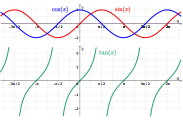
\includegraphics[width=0.8\columnwidth]{sincostan} 




\subsection{Parallelogrammgesetz}
\begin{theorem}
Sei $n \in \mathbb{N}_+$ und seien $v, w \in \mathbb{R}^n$ beliebig. Dann gilt:
\[
\|v + w\|^2 + \|v - w\|^2 = 2(\|v\|^2 + \|w\|^2)
\]
\end{theorem}

\begin{proof-example}
Wir berechnen direkt:
\begin{align*}
\|v + w\|^2 + \|v - w\|^2 &= (v+w)^T(v+w) + (v-w)^T(v-w) \\
&= v^Tv + 2v^Tw + w^Tw + v^Tv - 2v^Tw + w^Tw \\
&= 2v^Tv + 2w^Tw \\
&= 2(\|v\|^2 + \|w\|^2)
\end{align*}
\end{proof-example}

\subsection{Schiefsymmetrische Matrizen}
\begin{theorem}
Sei $n \in \mathbb{N}_+$ und sei $S \in \mathbb{R}^{n \times n}$ eine Matrix mit $S^T = -S$. Dann gilt $x^TSx = 0$ für alle $x \in \mathbb{R}^n$.
\end{theorem}

\begin{proof-example}
Für beliebiges $x \in \mathbb{R}^n$ gilt:
\begin{align*}
x^TSx &= (x^TSx)^T \quad \text{(da Skalar)} \\
&= x^TS^Tx \\
&= x^T(-S)x \quad \text{(da } S^T = -S) \\
&= -x^TSx
\end{align*}
Daraus folgt $x^TSx = -x^TSx$, also $2x^TSx = 0$ und somit $x^TSx = 0$.
\end{proof-example}

\subsection{Lineare Abhängigkeit von vier Vektoren in $\mathbb{R}^2$}
\begin{theorem}
Seien $u, v, w, z \in \mathbb{R}^2$ beliebig. Dann existieren Skalare $c_u, c_v, c_w, c_z \in \mathbb{R}$ mit mindestens einem $c_i \neq 0$, sodass
\[
c_u + c_v + c_w + c_z = 0 \quad \text{und} \quad c_uu + c_vv + c_ww + c_zz = 0.
\]
\end{theorem}

\begin{proof-example}
Da $\dim(\mathbb{R}^2) = 2$, sind vier Vektoren in $\mathbb{R}^2$ stets linear abhängig. Es existieren also Skalare $c_u, c_v, c_w, c_z \in \mathbb{R}$, nicht alle gleich Null, mit
\[
c_uu + c_vv + c_ww + c_zz = 0.
\]

Falls $c_u + c_v + c_w + c_z = 0$ bereits gilt, sind wir fertig.

Andernfalls sei $s := c_u + c_v + c_w + c_z \neq 0$. Definiere neue Koeffizienten:
\[
c'_u := c_u - \frac{s}{4}, \quad c'_v := c_v - \frac{s}{4}, \quad c'_w := c_w - \frac{s}{4}, \quad c'_z := c_z - \frac{s}{4}
\]

Dann gilt:
\[
c'_u + c'_v + c'_w + c'_z = (c_u + c_v + c_w + c_z) - s = 0
\]

Und:
\begin{align*}
c'_uu + c'_vv + c'_ww + c'_zz \\
= (c_uu + c_vv + c_ww + c_zz) - \frac{s}{4}(u + v + w + z) \\
= 0 - \frac{s}{4}(u + v + w + z) \\
= -\frac{s}{4}(u + v + w + z)
\end{align*}

Nicht alle $c'_i$ sind Null (da ihre Summe 0 ist, aber $s \neq 0$), womit die Behauptung bewiesen ist.
\end{proof-example}

\subsection{Linearität einer Funktion}
\begin{theorem}
Sei $n \in \mathbb{N}_+$. Die Funktion $f: \mathbb{R}^n \to \mathbb{R}$ definiert durch
\[
f(x) := \sum_{k=1}^n kx_k
\]
für alle $x = (x_1, x_2, \ldots, x_n)^T \in \mathbb{R}^n$ ist eine lineare Transformation.
\end{theorem}

\begin{proof-example}
Wir müssen zwei Eigenschaften zeigen:

\textbf{(1) Additivität:} Für beliebige $x, y \in \mathbb{R}^n$ gilt:
\begin{align*}
f(x + y) &= \sum_{k=1}^n k(x_k + y_k) = \sum_{k=1}^n (kx_k + ky_k) \\
&= \sum_{k=1}^n kx_k + \sum_{k=1}^n ky_k = f(x) + f(y)
\end{align*}

\textbf{(2) Homogenität:} Für beliebiges $x \in \mathbb{R}^n$ und $\lambda \in \mathbb{R}$ gilt:
\begin{align*}
f(\lambda x) &= \sum_{k=1}^n k(\lambda x_k) = \sum_{k=1}^n \lambda(kx_k) \\
&= \lambda \sum_{k=1}^n kx_k = \lambda f(x)
\end{align*}

Somit ist $f$ eine lineare Transformation.
\end{proof-example}

\subsection{Positive Definitheit und Eigenwerte}
\begin{theorem}
Seien $n \in \mathbb{N}_+$ und $S, T \in \mathbb{R}^{n \times n}$ symmetrisch und positiv definit. Falls es einen Vektor $v \in \mathbb{R}^n \setminus \{0\}$ und ein $\lambda \in \mathbb{R}$ gibt mit $STv = \lambda v$, dann gilt $\lambda > 0$.
\end{theorem}

\begin{proof-example}
Da $STv = \lambda v$ gilt:
\[
v^TSTv = v^T(\lambda v) = \lambda v^Tv = \lambda \|v\|^2
\]

Da $T$ symmetrisch und positiv definit ist, gilt $v^TTv > 0$ für alle $v \neq 0$.

Sei $w := Tv \neq 0$ (da $T$ positiv definit also invertierbar ist und $v \neq 0$).

Dann gilt:
\[
v^TSTv = w^TSw > 0
\]
da $S$ positiv definit ist und $w \neq 0$.

Somit folgt $\lambda \|v\|^2 > 0$, und da $\|v\|^2 > 0$ (weil $v \neq 0$), muss $\lambda > 0$ gelten.
\end{proof-example}

\subsection{Invertierbarkeit von $I + B$}
\begin{theorem}
Sei $n \in \mathbb{N}_+$ und $A := I + B$ mit $I \in \mathbb{R}^{n \times n}$ Identitätsmatrix und $B \in \mathbb{R}^{n \times n}$ mit $B_{ij} = 1$ für alle $i,j \in \{1,\ldots,n\}$. Dann ist $A$ invertierbar.
\end{theorem}

\begin{proof-example}
Wir zeigen, dass $\det(A) \neq 0$.

Betrachte $B$: alle Einträge sind 1, also $B = \mathbf{1}\mathbf{1}^T$ wobei $\mathbf{1} = (1,1,\ldots,1)^T$.

Die Matrix $B$ hat Rang 1 mit Eigenwert $n$ (zum Eigenvektor $\mathbf{1}$) und Eigenwert 0 mit Vielfachheit $n-1$.

Somit hat $A = I + B$ die Eigenwerte:
\begin{itemize}
\item $\lambda_1 = 1 + n$ (mit Eigenvektor $\mathbf{1}$)
\item $\lambda_2 = \ldots = \lambda_n = 1 + 0 = 1$ (mit Vielfachheit $n-1$)
\end{itemize}

Da alle Eigenwerte ungleich Null sind, gilt:
\[
\det(A) = (1+n) \cdot 1^{n-1} = 1 + n > 0
\]

Also ist $A$ invertierbar.
\end{proof-example}



\subsection{Nicht-Untervektorraum}
\begin{theorem}
Sei $n \in \mathbb{N}_+$ und $w \in \mathbb{R}^n$ mit $w \neq 0$. Dann ist die Menge
\[
S = \{v \in \mathbb{R}^n : v^Tw \leq 0\}
\]
kein Untervektorraum von $\mathbb{R}^n$.
\end{theorem}

\begin{proof-example}
Wir zeigen, dass $S$ nicht abgeschlossen unter Addition ist.

Da $w \neq 0$, existiert $i$ mit $w_i \neq 0$. Sei $e_i$ der $i$-te Standardbasisvektor.

Setze $v := -e_i$ falls $w_i > 0$, oder $v := e_i$ falls $w_i < 0$.

Dann gilt $v^Tw = -w_i < 0$ oder $v^Tw = w_i < 0$, also $v \in S$.

Aber: $v + v = 2v$ und
\[
(2v)^Tw = 2(v^Tw) < 0
\]

Allerdings: $v^Tw \leq 0$ und $v^Tw \leq 0$, aber für $\lambda = -1$ gilt:
\[
(\lambda v)^Tw = -v^Tw \geq 0
\]

Falls $v^Tw < 0$, dann ist $(-v)^Tw = -v^Tw > 0$, also $-v \notin S$.

Da $S$ nicht abgeschlossen unter Skalarmultiplikation ist, ist $S$ kein Untervektorraum.
\end{proof-example}

\subsection{Ungleichung mit Minimum}
\begin{theorem}
Seien $n \in \mathbb{N}_+$ und $v, w \in \mathbb{R}^n$ Vektoren mit nicht-negativen Einträgen, d.h. $v_i \geq 0$ und $w_i \geq 0$ für alle $i \in \{1,\ldots,n\}$. Definiere $u_i := \min\{v_i, w_i\}$ für alle $i$ und $u := (u_1, \ldots, u_n)^T$. Dann gilt:
\[
v \cdot w \geq \|u\|^2
\]
\end{theorem}

\begin{proof-example}
Für jedes $i \in \{1,\ldots,n\}$ gilt nach Definition von $u_i$:
\[
u_i \leq v_i \quad \text{und} \quad u_i \leq w_i
\]

Multipliziere diese Ungleichungen:
\[
u_i^2 \leq v_i w_i
\]

Summiere über alle $i$:
\[
\sum_{i=1}^n u_i^2 \leq \sum_{i=1}^n v_i w_i
\]

Dies ist äquivalent zu $\|u\|^2 \leq v \cdot w$.
\end{proof-example}

\subsection{Dimension des Untervektorraums}
\begin{theorem}
Sei $U = \{A \in \mathbb{R}^{2 \times 2} : \text{Tr}(A) = 0\}$ die Menge aller $2 \times 2$ Matrizen mit Spur 0. Dann gilt $\dim(U) = 3$.
\end{theorem}

\begin{proof-example}
Betrachte die Matrizen:
\[
B_1 = \begin{pmatrix} 1 & 0 \\ 0 & -1 \end{pmatrix}, \quad
B_2 = \begin{pmatrix} 0 & 1 \\ 0 & 0 \end{pmatrix}, \quad
B_3 = \begin{pmatrix} 0 & 0 \\ 1 & 0 \end{pmatrix}
\]

Alle drei haben Spur 0, also $B_1, B_2, B_3 \in U$.

\textbf{Lineare Unabhängigkeit:} Angenommen $c_1B_1 + c_2B_2 + c_3B_3 = 0$:
\[
\begin{pmatrix} c_1 & c_2 \\ c_3 & -c_1 \end{pmatrix} = \begin{pmatrix} 0 & 0 \\ 0 & 0 \end{pmatrix}
\]
Daraus folgt $c_1 = c_2 = c_3 = 0$.

\textbf{Erzeugnis:} Jede Matrix $A = \begin{pmatrix} a & b \\ c & d \end{pmatrix}$ mit $a + d = 0$ (also $d = -a$) lässt sich schreiben als:
\[
A = aB_1 + bB_2 + cB_3
\]

Also ist $\{B_1, B_2, B_3\}$ eine Basis von $U$ und $\dim(U) = 3$.
\end{proof-example}

\subsection{Symmetrie unter speziellen Bedingungen}
\begin{theorem}
Sei $n \in \mathbb{N}_+$ und $A \in \mathbb{R}^{n \times n}$ mit $AA^T = I$ und $A^2 = I$. Dann ist $A$ symmetrisch.
\end{theorem}

\begin{proof-example}
Aus $A^2 = I$ folgt $A = A^{-1}$.

Aus $AA^T = I$ folgt $A^T = A^{-1}$.

Also gilt $A = A^T$, d.h. $A$ ist symmetrisch.
\end{proof-example}

\subsection{Singulärwerte und Inverse}
\begin{theorem}
Sei $n \in \mathbb{N}_+$ und $A \in \mathbb{R}^{n \times n}$ invertierbar mit Inverse $A^{-1}$. Sei $\sigma_1$ der größte Singulärwert von $A$ und $\sigma'_1$ der größte Singulärwert von $A^{-1}$. Dann gilt:
\[
\sigma_1 \sigma'_1 \geq 1
\]
\end{theorem}

\begin{proof-example}
Sei $\sigma_n$ der kleinste Singulärwert von $A$.

Aus der Theorie wissen wir, dass die Singulärwerte von $A^{-1}$ gleich $\frac{1}{\sigma_i}$ sind (in umgekehrter Reihenfolge).

Also ist $\sigma'_1 = \frac{1}{\sigma_n}$.

Da $\sigma_1 \geq \sigma_n > 0$ (weil $A$ invertierbar ist), folgt:
\[
\sigma_1 \sigma'_1 = \sigma_1 \cdot \frac{1}{\sigma_n} \geq \frac{\sigma_n}{\sigma_n} = 1
\]
\end{proof-example}

\subsection{Cauchy-Schwarz Anwendung}
\begin{theorem}
Seien $n \in \mathbb{N}_+$ und $a_1, \ldots, a_n, b_1, \ldots, b_n \in \mathbb{R}$ mit $b_i > 0$ für alle $i$. Dann gilt:
\[
\sum_{i=1}^n \frac{a_i^2}{b_i} \geq \frac{(a_1 + \cdots + a_n)^2}{b_1 + \cdots + b_n}
\]
\end{theorem}

\begin{proof-example}
Definiere die Vektoren:
\[
u = \left( \frac{a_1}{\sqrt{b_1}}, \ldots, \frac{a_n}{\sqrt{b_n}} \right)^T, \quad
v = \left( \sqrt{b_1}, \ldots, \sqrt{b_n} \right)^T
\]

Nach Cauchy-Schwarz gilt $\|u\| \|v\| \geq |u \cdot v|$, also:
\[
\|u\|^2 \|v\|^2 \geq (u \cdot v)^2
\]

Berechne:
\begin{align*}
\|u\|^2 &= \sum_{i=1}^n \frac{a_i^2}{b_i} \\
\|v\|^2 &= \sum_{i=1}^n b_i \\
u \cdot v &= \sum_{i=1}^n \frac{a_i}{\sqrt{b_i}} \cdot \sqrt{b_i} = \sum_{i=1}^n a_i
\end{align*}

Einsetzen ergibt:
\[
\left(\sum_{i=1}^n \frac{a_i^2}{b_i}\right) \left(\sum_{i=1}^n b_i\right) \geq \left(\sum_{i=1}^n a_i\right)^2
\]

Division durch $\sum_{i=1}^n b_i > 0$ liefert die Behauptung.
\end{proof-example}

%%%%%%%%%%%%%%%%%%%%%%%%%%%%%%%%%%%%%%%%%%%%%
\section{\textcolor{teal}{Example Matrices}}
%%%%%%%%%%%%%%%%%%%%%%%%%%%%%%%%%%%%%%%%%%%%%
\setlength{\parindent}{0pt} % Fixes the "space at the left" issue

% --- Symmetric Matrices ---
\textbf{Symmetric} ($A = A^\top$): $\lambda_i \in \mathbb{R}$. Distinct eigenvectors orthogonal.
\begin{itemize}
    \item $2 \times 2$: $A = \begin{bmatrix} 1 & 2 \\ 2 & 1 \end{bmatrix} \implies \det = -3, \text{Tr} = 2, \lambda = \{3, -1\}$
    \item $3 \times 3$: $A = \begin{bmatrix} 2 & -1 & 0 \\ -1 & 2 & -1 \\ 0 & -1 & 2 \end{bmatrix} \implies \det = 4, \text{Tr} = 6, \lambda = \{2, 2 \pm \sqrt{2}\}$ (PSD)
\end{itemize}

\smallskip % Adds a tiny bit of space between categories

% --- Skew-Symmetric Matrices ---
\textbf{Skew-Symmetric} ($A = -A^\top$): $\text{Tr} = 0, \lambda = 0$ or imaginary. $\det=0$ if $n$ is odd.
\begin{itemize}
    \item $2 \times 2$: $A = \begin{bmatrix} 0 & 1 \\ -1 & 0 \end{bmatrix} \implies \det = 1, \lambda = \{i, -i\}$
    \item $3 \times 3$: $A = \begin{bmatrix} 0 & 1 & 2 \\ -1 & 0 & 3 \\ -2 & -3 & 0 \end{bmatrix} \implies \det = 0, \lambda = \{0, \pm i\sqrt{14}\}$
\end{itemize}

\smallskip

% --- Orthogonal Matrices ---
\textbf{Orthogonal} ($Q^\top Q = I$): $\det = \pm 1, |\lambda_i| = 1$. Preserves $\|x\|$ and $\angle(x,y)$.
\begin{itemize}
    \item $2 \times 2$ (Rot): $Q = \frac{1}{\sqrt{2}}\begin{bmatrix} 1 & -1 \\ 1 & 1 \end{bmatrix} \implies \det = 1, \lambda = \{e^{i\pi/4}, e^{-i\pi/4}\}$
    \item $3 \times 3$ (Perm): $P = \begin{bmatrix} 0 & 1 & 0 \\ 0 & 0 & 1 \\ 1 & 0 & 0 \end{bmatrix} \implies \det = 1, \lambda = \{1, e^{i2\pi/3}, e^{i4\pi/3}\}$
\end{itemize}

\smallskip

% --- Nilpotent Matrices ---
\textbf{Nilpotent} ($A^k = 0$): All $\lambda = 0 \implies \det = 0, \text{Tr} = 0$.
\begin{itemize}
    \item $2 \times 2$: $A = \begin{bmatrix} 0 & 1 \\ 0 & 0 \end{bmatrix} \implies A^2 = 0, \text{only one eigenvector } v = (1, 0)^\top$
    \item $3 \times 3$: $A = \begin{bmatrix} 0 & 1 & 2 \\ 0 & 0 & 3 \\ 0 & 0 & 0 \end{bmatrix} \implies A^3 = 0, \lambda = \{0, 0, 0\}$
\end{itemize}

\smallskip

% --- Diagonally Dominant Matrices ---
\textbf{Diagonally Dominant} ($|a_{ii}| > \sum_{j \neq i} |a_{ij}|$): Always invertible ($\det \neq 0$).
\begin{itemize}
    \item $3 \times 3$: $A = \begin{bmatrix} 3 & 1 & 1 \\ 1 & 4 & 2 \\ 0 & 1 & 2 \end{bmatrix} \implies \text{Row 1: } 3 > 1+1, \text{ Row 2: } 4 > 1+2$
\end{itemize}

\smallskip

% --- Rank-1 Matrices ---
\textbf{Rank-1} ($A = uv^\top$): $\text{rank}=1, \lambda = \{u^\top v, 0, \dots, 0\}$.
\begin{itemize}
    \item $3 \times 3$: $A = \begin{bmatrix} 1 & 1 & 1 \\ 2 & 2 & 2 \\ 3 & 3 & 3 \end{bmatrix} \implies \text{Tr} = 6, \lambda = \{6, 0, 0\}, \det = 0$
\end{itemize}

\smallskip

% --- Projection Matrices ---
\textbf{Projection} ($P^2 = P$): $\lambda \in \{0, 1\}$. $\text{rank}(P) = \text{Tr}(P)$.
\begin{itemize}
    \item $3 \times 3$: $P = \begin{bmatrix} 1 & 0 & 0 \\ 0 & 1 & 0 \\ 0 & 0 & 0 \end{bmatrix} \implies \lambda = \{1, 1, 0\}, \text{rank} = 2, \text{Tr} = 2$
\end{itemize}

\subsection{Transformations of $\mathbb{R}^2$}
Examples for linear transformations from $\mathbb{R}^2$ to itself, corresponding to square matrices $A\in \mathbb{R}^{2\times 2}$:
    $$A = 
    \begin{bmatrix}
        1 & 0 \\
        0 & 2
    \end{bmatrix}$$
    corresponds to \textbf{stretching} by a factor of 2 in the vertical axis. \\
    $$A = 
    \begin{bmatrix}
        1 & 0 \\
        1 & 1
    \end{bmatrix}$$
    corresponds to a \textbf{shearing} transformation. \\
    $$A = 
    \begin{bmatrix}
        \frac{1}{\sqrt2} & -\frac{1}{\sqrt2} \\
        \frac{1}{\sqrt2} & \frac{1}{\sqrt2}
    \end{bmatrix}$$
    corresponds to a counter-clockwise \textbf{rotation} by $\frac{\pi}{4}$. \\

    $$A = 
    \begin{bmatrix}
        0 & 1 \\
        1 & 0
    \end{bmatrix}$$
    corresponds to a \textbf{reflection} by the diagonal line $x_2 = x_1$. \\


\subsection*{1. Symmetrisch}
$\begin{pmatrix}2&1\\1&3\end{pmatrix}$ 
$\begin{pmatrix}1&2&0\\2&3&1\\0&1&4\end{pmatrix}$\\
\nullyes{} \quad \textit{$A=A^\top$}

\subsection*{2. Orthogonal}
$\begin{pmatrix}0&1\\1&0\end{pmatrix}$ 
$\begin{pmatrix}1&0&0\\0&0&1\\0&1&0\end{pmatrix}$\\
\nullno{} \quad \textit{$Q^\top Q=I$}

\subsection*{3. Positiv definit}
$\begin{pmatrix}2&1\\1&2\end{pmatrix}$ 
$\begin{pmatrix}2&1&0\\1&2&1\\0&1&2\end{pmatrix}$\\
\nullno{} \quad \textit{$\lambda_i>0$}

\subsection*{4. Diagonal}
$\begin{pmatrix}3&0\\0&5\end{pmatrix}$ 
$\begin{pmatrix}2&0&0\\0&4&0\\0&0&6\end{pmatrix}$\\
\nullyes{} \quad \textit{Nur Diagonale}

\subsection*{5. Obere Dreiecks}
$\begin{pmatrix}1&2\\0&3\end{pmatrix}$ 
$\begin{pmatrix}1&2&3\\0&4&5\\0&0&6\end{pmatrix}$\\
\nullyes{} \quad \textit{Unter Diag. = 0}

\subsection*{6. Untere Dreiecks}
$\begin{pmatrix}2&0\\3&1\end{pmatrix}$ 
$\begin{pmatrix}1&0&0\\2&3&0\\4&5&6\end{pmatrix}$\\
\nullyes{} \quad \textit{Über Diag. = 0}

\subsection*{7. Strikt diag. dom.}
$\begin{pmatrix}3&1\\1&4\end{pmatrix}$ 
$\begin{pmatrix}4&1&1\\1&5&2\\1&1&6\end{pmatrix}$\\
\nullno{} \quad \textit{$|a_{ii}|>\sum_{j\neq i}|a_{ij}|$}

\subsection*{8. Singulär}
$\begin{pmatrix}1&2\\2&4\end{pmatrix}$ 
$\begin{pmatrix}1&2&3\\2&4&6\\1&2&3\end{pmatrix}$\\
\nullyes{} \quad \textit{$\det=0$}

\subsection*{9. Idempotent}
$\begin{pmatrix}1&0\\0&0\end{pmatrix}$ 
$\begin{pmatrix}1&0&0\\0&1&0\\0&0&0\end{pmatrix}$\\
\nullyes{} \quad \textit{$A^2=A$}

\subsection*{10. Nilpotent}
$\begin{pmatrix}0&1\\0&0\end{pmatrix}$ 
$\begin{pmatrix}0&1&0\\0&0&1\\0&0&0\end{pmatrix}$\\
\nullyes{} \quad \textit{$N^k=0$}

\subsection*{11. Invertierbar}
$\begin{pmatrix}1&2\\3&4\end{pmatrix}$ 
$\begin{pmatrix}1&0&1\\0&2&0\\1&0&2\end{pmatrix}$\\
\nullno{} \quad \textit{$\det\neq 0$}

\subsection*{12. Tridiagonal}
$\begin{pmatrix}2&1\\1&2\end{pmatrix}$ 
$\begin{pmatrix}2&1&0\\1&2&1\\0&1&2\end{pmatrix}$\\
\nullyes{} \quad \textit{3 Diagonalen}

\subsection*{13. Rang-1}
$\begin{pmatrix}1&2\\2&4\end{pmatrix}$ 
$\begin{pmatrix}1&2&3\\2&4&6\\1&2&3\end{pmatrix}$\\
\nullno{} \quad \textit{rank=1}

\subsection*{15. Schiefsymmetrisch}
$\begin{pmatrix}0&1\\-1&0\end{pmatrix}$ 
$\begin{pmatrix}0&1&2\\-1&0&3\\-2&-3&0\end{pmatrix}$\\
\nullyes{} \quad \textit{$A^\top=-A$}

\subsection*{16. Eigenwerte $\gt$ 0}
$\begin{pmatrix}1&2\\0&3\end{pmatrix}$ 
$\begin{pmatrix}1&1&0\\0&2&1\\0&0&3\end{pmatrix}$\\
\nullno{} \quad \textit{$\lambda_i>0$}

\subsection*{17. Eigenwerte $\lt$ 0}
$\begin{pmatrix}-1&2\\0&-3\end{pmatrix}$ 
$\begin{pmatrix}-1&1&0\\0&-2&1\\0&0&-3\end{pmatrix}$\\
\nullno{} \quad \textit{$\lambda_i<0$}

\subsection*{18. Positiv semidefinit}
$\begin{pmatrix}1&1\\1&1\end{pmatrix}$ 
$\begin{pmatrix}1&1&0\\1&1&0\\0&0&0\end{pmatrix}$\\
\nullyes{} \quad \textit{$\lambda_i\geq 0$}

\subsection*{19. Negativ definit}
$\begin{pmatrix}-2&-1\\-1&-2\end{pmatrix}$ 
$\begin{pmatrix}-2&-1&0\\-1&-2&-1\\0&-1&-2\end{pmatrix}$\\
\nullno{} \quad \textit{$\lambda_i<0$}

\subsection*{20. Hermitesch}
$\begin{pmatrix}2&1+i\\1-i&3\end{pmatrix}$ 
$\begin{pmatrix}1&i&0\\-i&2&1+i\\0&1-i&3\end{pmatrix}$\\
\nullyes{} \quad \textit{$H=H^*$}

\subsection*{21. Unitär}
$\begin{pmatrix}\frac{1}{\sqrt{2}}&\frac{i}{\sqrt{2}}\\\frac{i}{\sqrt{2}}&\frac{1}{\sqrt{2}}\end{pmatrix}$ 
$\begin{pmatrix}1&0&0\\0&\frac{1}{\sqrt{2}}&\frac{i}{\sqrt{2}}\\0&\frac{i}{\sqrt{2}}&\frac{1}{\sqrt{2}}\end{pmatrix}$\\
\nullno{} \quad \textit{$U^*U=I$}

\subsection*{22. Normal}
$\begin{pmatrix}1&1\\-1&1\end{pmatrix}$ 
$\begin{pmatrix}1&0&1\\0&2&0\\1&0&1\end{pmatrix}$\\
\nullyes{} \quad \textit{$AA^*=A^*A$}

\subsection*{23. Involutorisch}
$\begin{pmatrix}0&1\\1&0\end{pmatrix}$ 
$\begin{pmatrix}1&0&0\\0&0&1\\0&1&0\end{pmatrix}$\\
\nullno{} \quad \textit{$A^2=I$}

\subsection*{24. Permutation}
$\begin{pmatrix}0&1\\1&0\end{pmatrix}$ 
$\begin{pmatrix}0&1&0\\0&0&1\\1&0&0\end{pmatrix}$\\
\nullno{} \quad \textit{1 Eins/Zeile}



\end{small}

\end{multicols*}
\end{document}
